% mnras_template.tex 
%
% LaTeX template for creating an MNRAS paper
%
% v3.0 released 14 May 2015
% (version numbers match those of mnras.cls)
%
% Copyright (C) Royal Astronomical Society 2015
% Authors:
% Keith T. Smith (Royal Astronomical Society)

% Change log
%
% v3.0 May 2015
%    Renamed to match the new package name
%    Version number matches mnras.cls
%    A few minor tweaks to wording
% v1.0 September 2013
%    Beta testing only - never publicly released
%    First version: a simple (ish) template for creating an MNRAS paper

%%%%%%%%%%%%%%%%%%%%%%%%%%%%%%%%%%%%%%%%%%%%%%%%%%
% Basic setup. Most papers should leave these options alone.
\documentclass[fleqn,usenatbib]{mnras}

% MNRAS is set in Times font. If you don't have this installed (most LaTeX
% installations will be fine) or prefer the old Computer Modern fonts, comment
% out the following line
\usepackage{newtxtext,newtxmath}
% Depending on your LaTeX fonts installation, you might get better results with one of these:
% \usepackage{mathptmx}
% \usepackage{txfonts}

% Use vector fonts, so it zooms properly in on-screen viewing software
% Don't change these lines unless you know what you are doing
\usepackage[T1]{fontenc}

% Allow "Thomas van Noord" and "Simon de Laguarde" and alike to be sorted by "N" and "L" etc. in the bibliography.
% Write the name in the bibliography as "\VAN{Noord}{Van}{van} Noord, Thomas"
\DeclareRobustCommand{\VAN}[3]{#2}
\let\VANthebibliography\thebibliography
\def\thebibliography{\DeclareRobustCommand{\VAN}[3]{##3}\VANthebibliography}


%%%%% AUTHORS - PLACE YOUR OWN PACKAGES HERE %%%%%

% Only include extra packages if you really need them. Common packages are:
\usepackage{graphicx}	% Including figure files
\usepackage{amsmath}	% Advanced maths commands
% \usepackage{amssymb}	% Extra maths symbols

% Allow fractional font size
\usepackage{anyfontsize}

%%%%%%%%%%%%%%%%%%%%%%%%%%%%%%%%%%%%%%%%%%%%%%%%%%

%%%%% AUTHORS - PLACE YOUR OWN COMMANDS HERE %%%%%

% Please keep new commands to a minimum, and use \newcommand not \def to avoid
% overwriting existing commands. Example:
%\newcommand{\pcm}{\,cm$^{-2}$}	% per cm-squared

%%%%%%%%%%%%%%%%%%%%%%%%%%%%%%%%%%%%%%%%%%%%%%%%%%

%%%%%%%%%%%%%%%%%%% TITLE PAGE %%%%%%%%%%%%%%%%%%%

% Title of the paper, and the short title which is used in the headers.
% Keep the title short and informative.
\title[The Unified Cluster Catalogue]{The Unified Cluster Catalogue: towards a
comprehensive and homogeneous database of stellar clusters}

% The list of authors, and the short list which is used in the headers.
% If you need two or more lines of authors, add an extra line using \newauthor
\author[G. I. Perren et al.]{
Gabriel I. Perren,$^{1,3}$\thanks{E-mail: gabrielperren@gmail.com}
Mar\'ia S. Pera,$^{2,3}$
Hugo D. Navone$^{2,3}$
and Rub\'en A. V\'azquez$^{1,4}$
\\
% List of institutions
$^{1}$Instituto de Astrof\'isica de La Plata, IALP (CONICET-UNLP), 1900 La Plata, Argentina\\
$^{2}$Instituto de F\'isica de Rosario, IFIR (CONICET-UNR), 2000 Rosario, Argentina\\
$^{3}$Facultad de Ciencias Exactas, Ingenier\'ia y Agrimensura (UNR), 2000 Rosario, Argentina\\
$^{4}$Facultad de Ciencias Astron\'omicas y Geof\'isicas (UNLP), 1900 La Plata, Argentina
}


% These dates will be filled out by the publisher
\date{Accepted XXX. Received YYY; in original form ZZZ}

% Enter the current year, for the copyright statements etc.
\pubyear{2023}

% Don't change these lines
\begin{document}
\label{firstpage}
\pagerange{\pageref{firstpage}--\pageref{lastpage}}
\maketitle

% Abstract of the paper
% single paragraph not more than 250 words
\begin{abstract}
We present the Unified Cluster Catalogue, the largest catalogue of stellar
clusters with almost 14000 objects listed to date. In this initial
version only Milky Way open clusters are present, but other objects will be
included in the future. Each cluster is processed with a new probability
membership algorithm designed to incorporate each star's coordinates, parallax,
proper motions, and their uncertainties into the probability assignment process.
We employ Gaia DR3 data up to a G magnitude of 20, resulting in more than a
million probable members identified. The catalogue is accompanied by a public
web site aimed at facilitating the search and data exploration of stellar
clusters.
\end{abstract}

% Select between one and six entries from the list of approved keywords.
% Don't make up new ones.
\begin{keywords}
(Galaxy:) open clusters and associations: general --
catalogues -- methods: data analysis
\end{keywords}

%%%%%%%%%%%%%%%%%%%%%%%%%%%%%%%%%%%%%%%%%%%%%%%%%%

%%%%%%%%%%%%%%%%% BODY OF PAPER %%%%%%%%%%%%%%%%%%

\section{Introduction}

% Importance of open clusters
Open clusters (OCs) are groups of gravitationally bound coeval stars
with a wide range of masses, that formed from the same molecular cloud.
Their orbits generally locate them close to the Galactic disk, although there
are a few examples of OCs with large vertical distances. Having originated from
the same cloud, their member stars share a chemical composition and age, and are
located spanning a somewhat compact position in space.
The study of OCs is of fundamental importance for a number of key aspects in
astrophysics research, including the process of stellar evolution as well as the
dynamics, structure, formation, and chemical evolution of the
Galaxy~\citep{Friel1995}.

% Importance of catalogues
Catalogues of OCs are crucial not only to organize these objects into publicly
available systematic databases, but most importantly to assist researchers on the
task of discovering new potential objects and, almost equally important,
discard false detections.
Catalogued bonafide OCs are also the most natural training dataset against which
we can test and eventually improve new algorithms for stellar clusters
detection.
%
There have been efforts to provide catalogues of OCs to the astrophysical
research community at least since the late 18th century, even if that was not
the primary objective of the compilation. The first of such well known
catalogues to include OCs is the Messier Catalogue~\citep{Messier1771} with
less than 30 OCs listed. This work was quickly followed by Herschel's
Catalogue of One Thousand New Nebulae and Clusters of
Stars~\citep{Herschel1786}, culminating a century later with Dreyer's New
General Catalogue of Nebulae and Clusters of Stars~\citep[NGC,][]{Dreyer1888}.
The NGC lists less than 650 OCs, which is more than twenty times the number of
objects present in Messier's catalogue.
% NGC catalogue listing:
% https://in-the-sky.org/data/catalogue.php?cat=NGC&const=1&obj1Type=6&sort=0&view=1&page=6

After that first rapid growth, the pace with which OCs were discovered and
catalogued slowed down. The next big catalogue, again published almost a
century later, was the Base Données Amas~\citep{Mermilliod1995} which
listed a little over 1100 OCs, based on the previous compilation
by~\cite{Lynga1987}. This work is the foundation of the WEBDA
catalogue,\footnote{\url{https://webda.physics.muni.cz/webda.html}} a heavily
used resource in the analysis of OCs which currently lists almost 1800 objects.

In the following decade, with the advent of large public databases containing
from hundreds of thousands to millions of stars --- such as Hipparcos and
Tycho~\citep{Perryman_1997,Hog_1997} and 2MASS~\citep{Skrutskie_2006} --- the
task of detecting new candidate OCs became substantially more attainable. This
is particularly true for those objects that are faint, obscured by dust, or not
in the vicinity of the solar system. Catalogues such as the Milky Way Star
Clusters~\citep{Kharchenko_2012} or those presented
by~\cite{Loktin_2017} or~\cite{Bica_2019} increased the number of listed OCs to
more than 3000 in a few decades.

Finally in present time, the release of the database for the Gaia
survey~\citep{Gaia_2016} with over a billion observed stars, translated into an
enormous quantity of new candidate OCs reported in the literature. Clustering
algorithms such as HDBSCAN~\citep{Campello_2013} are used for the automatic
identification of overdensities, improving dramatically the detection
sensitivity compared to manual methods.
The latest published catalogue is the one presented in~\cite{Hunt_2023}
with $\sim$7000 listed OCs, $\sim$2000 of which are new candidates.

% What we do in this article
In this work we compiled a total of almost 14000 OCs, with about half of that
number being new candidates discovered just in the past two years.
As seen in Fig.~\ref{fig:catalogued_ocs} the growth in catalogued OCs
in the last two centuries is almost exponential and, taking the last few years
as a trend, it shows no sign of slowing down. Estimates for the total number
of OCs in the Galaxy locate the upper limit over 10$^{5}$, which means that
there remain still a lot of objects waiting to be found.
%
The problem with these massive studies where new candidate OCs are presented by
the thousands is simple: there are too many of them to be properly and
individually analysed. Depending on the parameters used for the clustering
algorithms employed, apparent groupings of non-physically related stars can
easily disguise themselves as OCs.
Furthermore, the scatter of information among dozens of articles and the influx
of new articles published just months apart means that authors are often times
not able to check their results against other catalogues; recent or not. This
translates into duplication issues which, combined with the aforementioned
problem, can have non trivial effects when these objects are used in massive
studies (for example, when analysing the Galactic structure).

\begin{figure}
	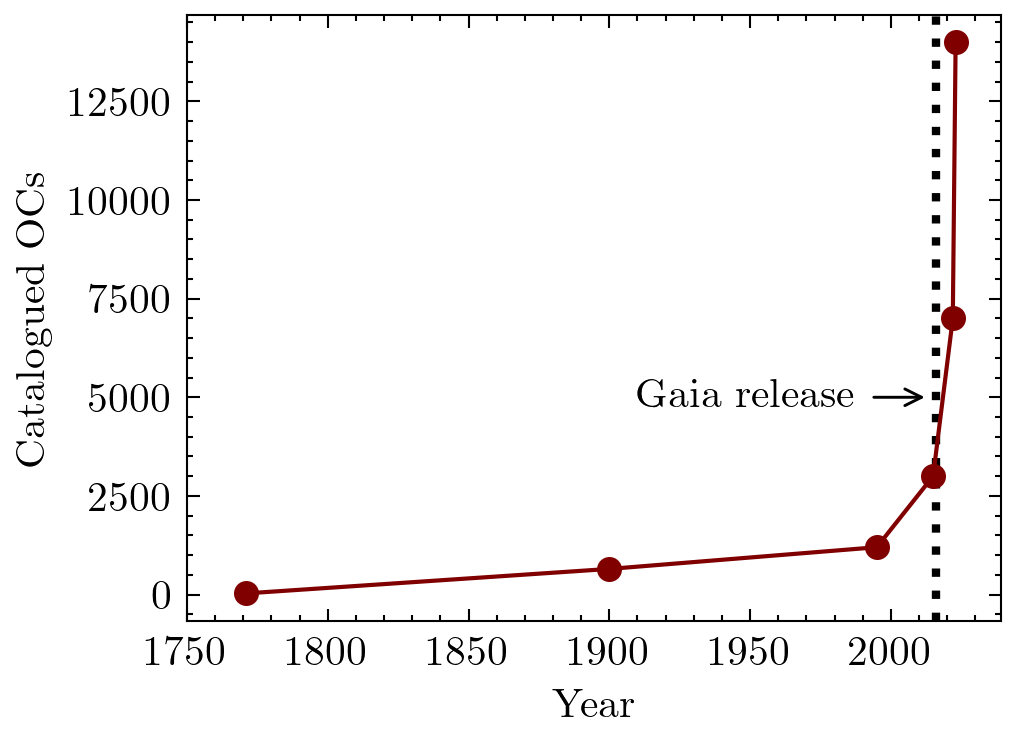
\includegraphics[width=\columnwidth]{figs/catalogued_ocs.png}
    \caption{Approximate number of catalogued OCs in the literature since the
    late 1700s to the present day (including this work). The date of the
    release of the Gaia's survey data is marked as a dotted line.}
    \label{fig:catalogued_ocs}
\end{figure}

Our aim is to provide the community with a service that can be used to
alleviate these issues. We combine --- to the best of our knowledge--- all the
recent catalogues of OCs in the literature, and use them to generate a single
unified catalogue of $\sim$14000 OCs. We call this the Unified Cluster Catalogue
(UCC hereafter), which can be accessed via the site
\href{https://ucc.ar/}{\texttt{ucc.ar}}.
We apply over each listed OC a new tool
to assign membership probabilities called \texttt{fastMP} (``fast Membership
Probability'').\footnote{\texttt{fastMP}:\url{https://github.com/Gabriel-p/fastMP}}
The code was designed to work on the Gaia survey data, resulting
so far in more than 1 million stars identified as probable members of the
catalogued OCs. This gives us the largest homogeneously processed
database of OC members to date. The data collected for each OC in the UCC
catalogue, along with their estimated members, is publicly available in the
aforementioned site. This site will be periodically updated as new candidate OCs
are presented to the community.

% Structure of the article
This article is structured as follows. In Sect.~\ref{sec:databases} we
introduce the stellar cluster databases employed to generate this initial
version of the combined catalogue. Section~\ref{sec:methods} presents the
new membership algorithm employed in the study of all the catalogued clusters.
A comparison of our membership results with those recently published is
performed in Sect.~\ref{sec:results}, along with the presentation of the public
web site where these results will be hosted, updated, and expanded in the future.
Finally, our conclusions are highlighted in Sect.~\ref{sec:conclusions}.


%%%%%%%%%%%%%%%%%%%%%%%%%%%%%%%%%%%%%%%%%%%%%%%%%%
\section{Databases}
\label{sec:databases}

We have gathered, to the best of our knowledge, all the recent OCs listed in
the literature up to present day. These were extracted from 32 databases that
were published in the last 11 years. The total number of entries is 24983,
cross-matched to a final catalogue of 13684 unique OCs.
A few small databases were not added individually as they are included entirely
in~\cite{Hunt_2023}: \cite{Zari_2018}, \cite{Bastian_2019}, \cite{Tian_2020}, 
\cite{Qin_2021}, \cite{Anders_2022}, \cite{Casado_2023}.
%
Table~\ref{tab:references} lists these works along with the number of OCs
that were left after extensive cleaning and sanitizing. To avoid cluttering the
article we mention the details in Appendix~\ref{app:db_cleaning}, and restrict
this section to a general discussion of the process.

\begin{table}
	\centering
	\caption{Catalogues used in this article to generate the combined final
	catalogue with 13684 entries. Columns ID and N are the denomination used for
	new candidate OCs presented in those works, and the total number of OCs
	taken from them, respectively. Abbreviations used throughout this
	article for two of the works are also shown.}
	\label{tab:references}
	\begin{tabular}{lcr}
		\hline
		% Reference & \verb|                              | N\\
		Reference & ID & N\\
		\hline
		\cite{Kharchenko_2012}  & -- & 2854\\
		\cite{Loktin_2017}   & LP & 1050\\
		\cite{Castro_Ginard_2018} & UBC   & 23\\
		\cite{Bica_2019} &  Bica  & 3555\\
		\cite{Castro-Ginard_2019}  & UBC & 53\\
		\cite{Sim_2019}  & UPK    & 207\\
		\cite{Liu_2019}  & FoF    & 76\\
		\cite{Ferreira_2019}  & UFMG   & 3\\
		\cite{Castro-Ginard_2020}  & UBC  & 570\\
		\cite{Ferreira_2020}  & UFMG  & 25\\
		\citet[][CANTAT20]{Cantat-Gaudin_2020} & --  & 2017\\
		\cite{Hao_2020}   & HXWHB  & 16\\
		\cite{Ferreira_2021}  & UFMG   & 34\\
		\cite{He_2021}  & HXHWL  & 74\\
		\cite{Dias_2021}  &  --  & 1742\\
		\cite{Hunt_2021}  & PHOC  & 41\\
		\cite{Casado_2021}  & Casado  & 20\\
		\cite{Jaehnig_2021}   & XDOCC   & 11\\
		\cite{Santos-Silva_2021}  & CMa   & 5\\
		\cite{Tarricq_2022}   & --  & 467\\
		\cite{Castro-Ginard_2022} & UBC  & 628\\
		\cite{He_2022}  & CWNU  & 541\\
		\cite{He_2022_1}   & CWNU  & 836\\
		\cite{Hao_2022}  & OC   & 703\\
		\cite{Li_2022}  & LISC   & 61\\
		\cite{He_2023}  & CWNU   & 1656\\
		\citet[][HUNT23]{Hunt_2023}   & HSC  & 6272\\
		\cite{Qin_2023}  & OCSN    & 101\\
		\cite{Li_2023}  & LISC  & 35\\
		\cite{Chi_2023_2} & CWWL  & 46\\
		\cite{Chi_2023}  & LISC-III    & 82\\
		\cite{Chi_2023_3}  & CWWDL  & 1179\\
		\hline
		Total OCs in combined catalogues    &   & 24983\\
		Total unique OCs after cross-matching  &  & 13684\\
		\hline
	\end{tabular}
\end{table}

Unlike other works such as the recent HUNT23, we do not attempt to cross-match
the OCs listed in different databases using positions and/or astrometry.
Instead, we standardize the names of all the catalogued OCs and combine their
parameters when present in multiple catalogues.
This name-based matching means that if an OC is listed with more than one
denomination in a given database, this will be carried out and added to the
rest of the catalogues where it is found. Although we do not attempt to find
duplicate OCs via positions and/or astrometry cross-matching, we do use this
data to flag the most obvious duplicate entries. For example, the CWWDL 14677
candidate OC presented in~\cite{Chi_2023_3}, has coordinates and astrometry
values estimated as: RA=0.9526\textdegree, DEC=-30.002\textdegree, pmRA=4.222 
mas yr$^{-1}$, pmDE=18.721 mas yr$^{-1}$, plx=2.61 mas. This is marked in the
UCC as a duplicate of the well known Blanco 1 OC which has almost identical
coordinates and astrometry values in the literature: RA=0.9149\textdegree,
DEC=-29.958\textdegree, pmRA=4.215 mas yr$^{-1}$, pmDE=18.724 mas yr$^{-1}$, and 
plx=2.59 mas. There are many entries with similar issues. Note that although
cases such as this one are flagged as possible duplicates, they are not
removed from the final catalogue. The reasoning behind this is that the authors
presented these objects as new findings, and we maintain this denomination. Even
if the duplication is very clear, we believe that this decision can help
future research in identifying structures that were wrongly tagged as
unique OCs, and avoid repeating the same mistake. It can also aid in the
detection and analysis of binary cluster systems.
We will show in Sect.~\ref{sec:results} how each OC is assigned a probability of
being a duplicate of others in the catalogue, based on a simple set of rules.
This classification, even if not rigorous, is a very reasonable first step in a
deeper analysis about duplication of candidates OCs in the literature.

\begin{figure*}
	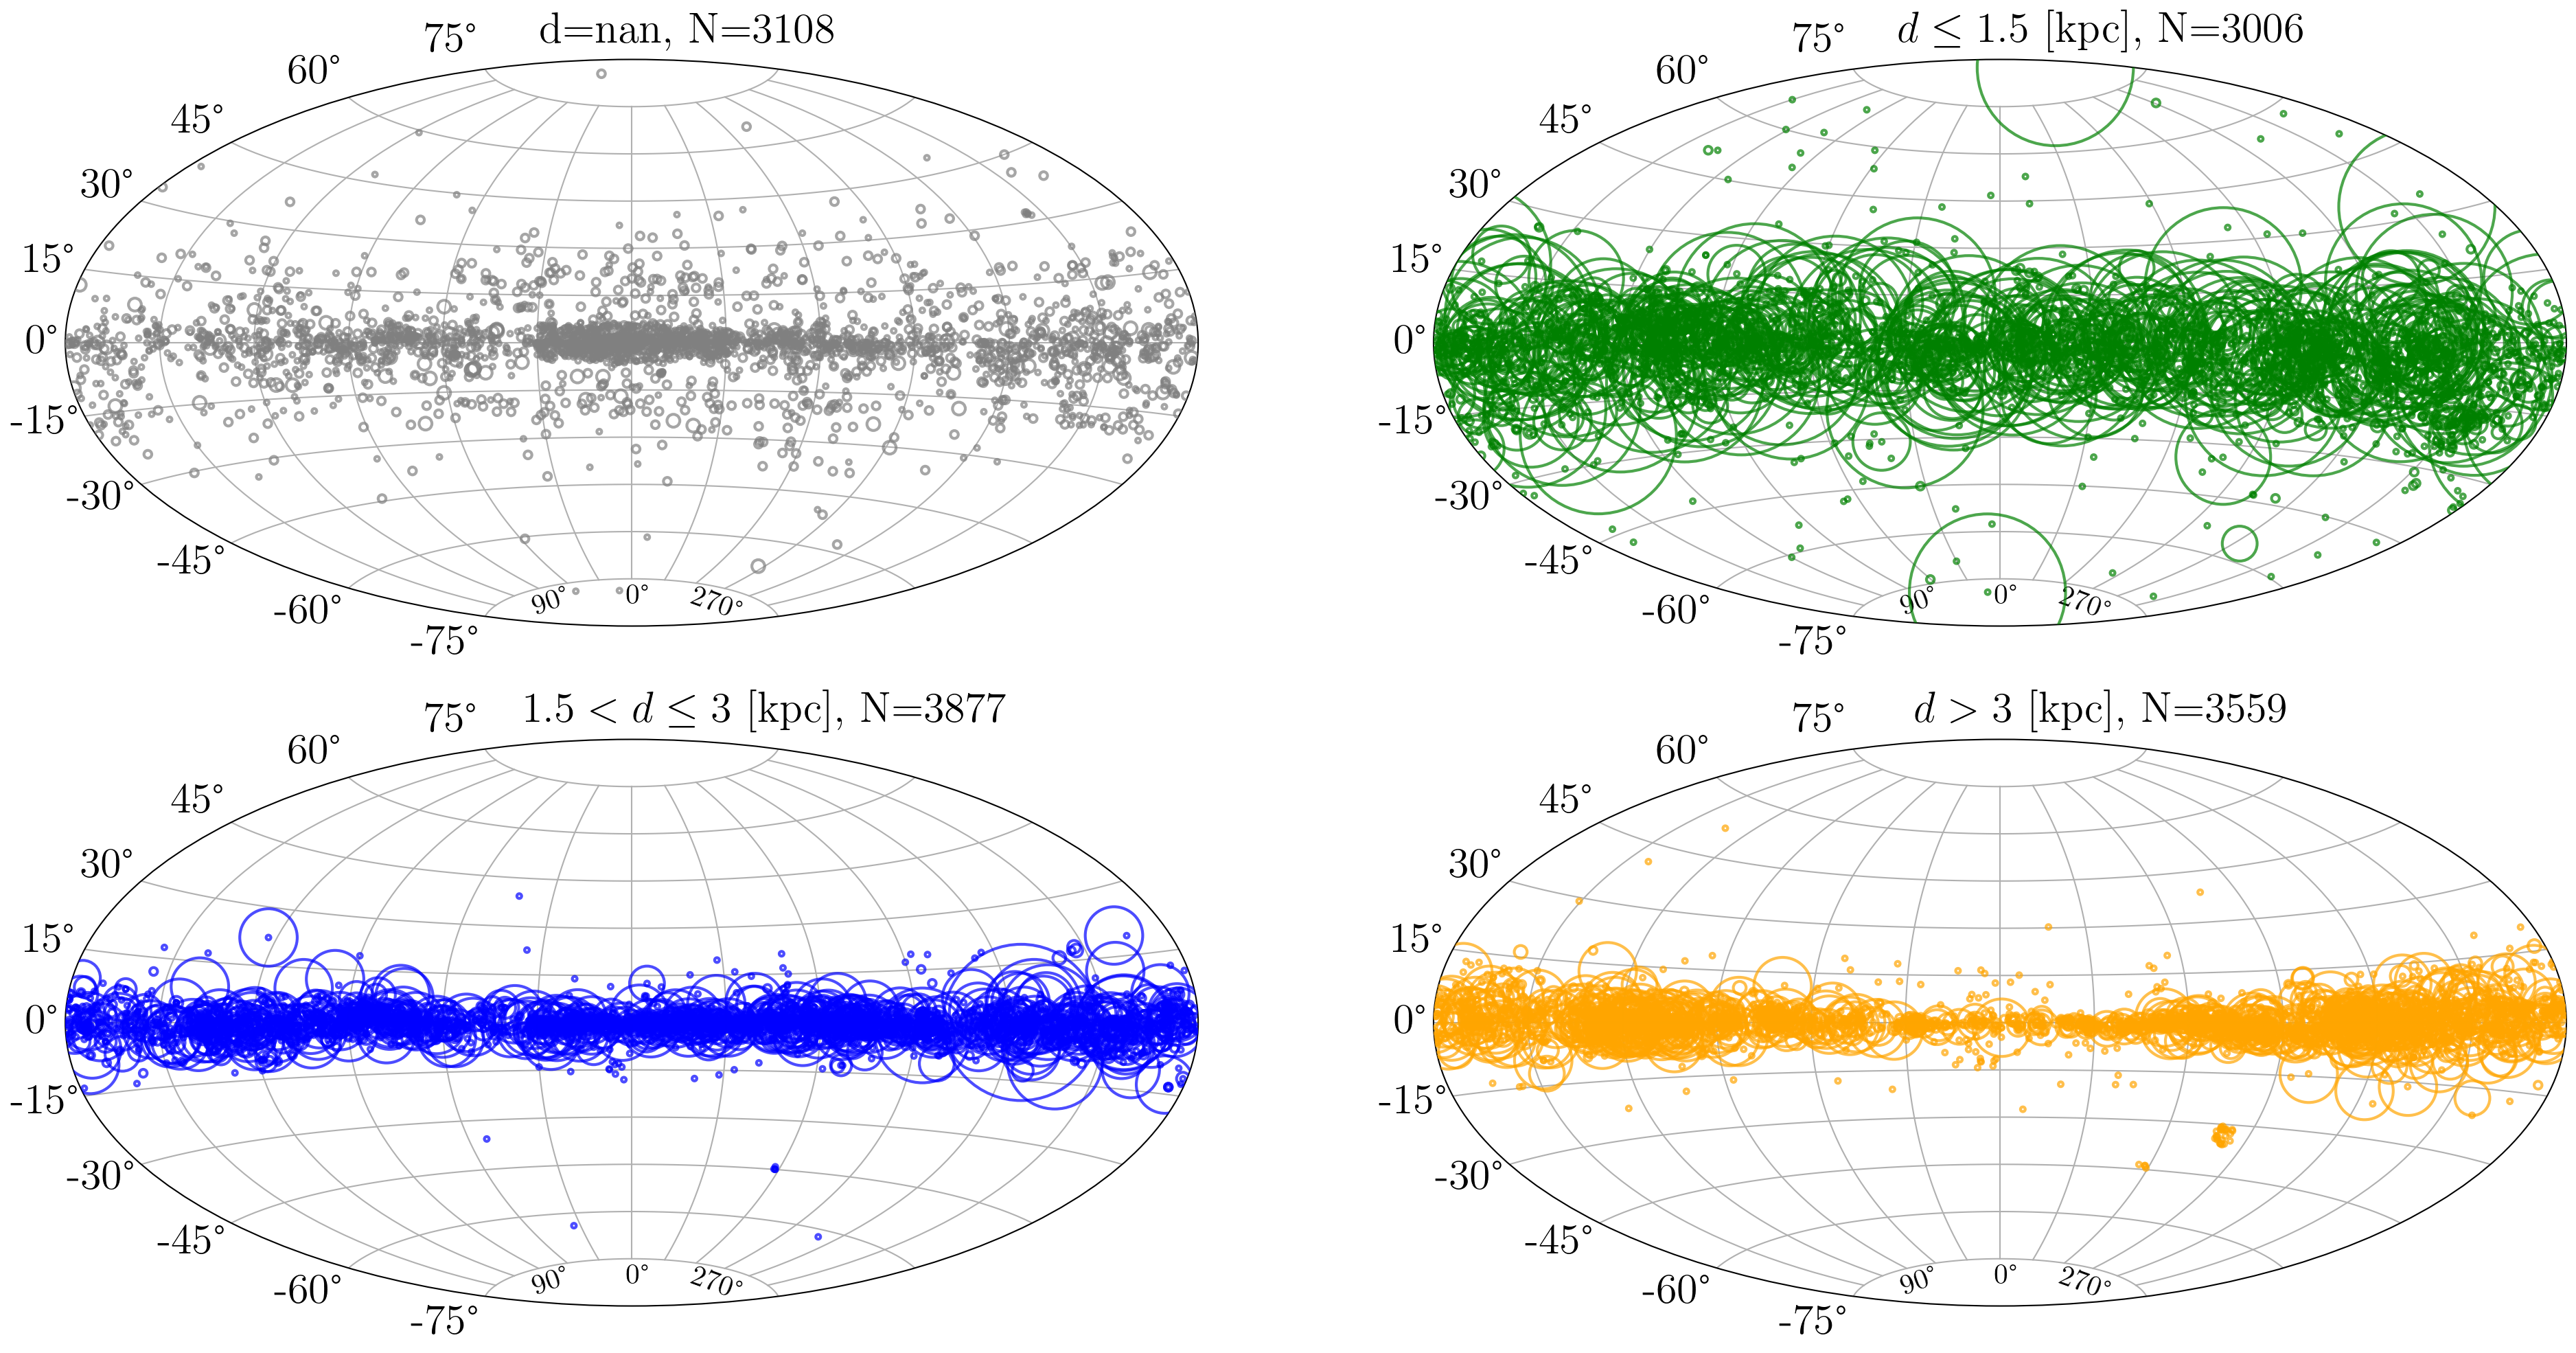
\includegraphics[width=\textwidth]{figs/galactic_map.png}
    \caption{Map of the full list of catalogued OCs in this work, in
    galactic coordinates, by range of catalogued distance. From top left
    to bottom right: OCs catalogued with no distance (grey), OCs with
    $d\leq1.5$ kpc (green), OCs in the range $1.5<d\leq3$ kpc (blue), and OCs
    with $d>3$ kpc (orange). Sizes are proportional to the number of
    databases from Table~\ref{tab:references} that include the candidate OC.}
    \label{fig:galactic_map}
\end{figure*}

In Fig.~\ref{fig:galactic_map} we show the distribution of the 13684 OC
candidates catalogued in the UCC so far, segregated by distance range. These
distances are estimated as the inverse of the listed parallaxes. It is worth
noting that many of the OCs in older catalogues, such
as~\cite{Kharchenko_2012} and~\cite{Bica_2019}, have
no associated astrometry but can have distances estimated as part of the
fundamental parameters analysis process (usually along with age and extinction).
As seen in the top left plot, these catalogued OCs with no astrometry represent
almost a quarter of the database.
Expectedly, those OCs catalogued closer than $\sim$1.5 kpc (right top plot) are
listed in many more databases than the rest (as shown by the proportional sizes
of the circles).

The UCC includes candidate OCs found through analysis of infrared
photometry such as the FSR~\citep{Froebrich_2007}, Ryu~\citep{Ryu_2018}, and
VVV~\citep{Barba_2015} objects. These have not been included in any of the
recent large scale analysis like CANTAT20 and HUNT23 because they are considered
to be too obscure for Gaia photometry. A large portion of the OCs with no
astrometry seen in the top left panel of Fig.~\ref{fig:galactic_map} are
precisely these objects.
Our method, as we will show in Sect~\ref{sec:methods}, does not depend on the
ability of a clustering algorithm to detect a faint and small overdensity, which
it will most likely not be able to accomplish. Thus, we can include these OCs
here and report a first approximation of their mean positions in proper motions
and parallax.

In this initial version of the UCC we did not include information on
candidate OCs identified to be probable asterisms, as that presented for example
in~\cite{Cantat-Anders_2020}. This data is much more scattered and difficult to
collect but we plan on including it in future updates to the catalogue. This
fact notwithstanding, we do assign two different quality parameters to each
object which are very useful in the process of identifying probable
non-clusters. This will be discussed in more detail in Sect~\ref{sec:results}.

Recently~\cite{Kounkel_2020} presented a list of more than 8000 moving
groups. Many of these are very extended and small groups which
can hardly be classified as OCs. For this initial version of the UCC we remove
these groups from the catalogues where they are included, i.e.
\cite{He_2022_1} and HUNT23.\\
% Kounkel private communication:
% "*All of these populations are moving groups. The word "cluster" is so nebulous
% nowadays, we don't have a proper definition of what it means any more, outside
% of those classicaly identified.*"\\

While we were preparing this manuscript a new work by He et al. was presented
with $\sim$2000 new candidate OCs, whose associated data is still not fully
available~\cite{He_2023_2}. Although it is not included in the initial version
of the UCC presented here, it will most likely already be included by the time
this article is published (assuming the data is eventually made public).\\

Finally, we made use of the latest release of the Gaia survey data
(DR3)~\citep{GaiaDR3_2022,Babusiaux_2022} imposing a single cut on a maximum
magnitude of G=20 mag. No other filters were applied on this data which was
employed, as we will detail in Sect.~\ref{sec:methods}, to process the entire
catalogue extracting the most likely members for each listed OC.



% Gaia references:
% https://gea.esac.esa.int/archive/documentation/GDR3/Miscellaneous/sec_credit_and_citation_instructions/



%%%%%%%%%%%%%%%%%%%%%%%%%%%%%%%%%%%%%%%%%%%%%%%%%%
\section{Membership method}
\label{sec:methods}

Once the unified catalogue is generated, our next objective is to compile an
homogeneous database of likely member stars for each OC in the UCC.
Usually a handful of tools are employed for this task, referred to
as clustering algorithms. Three of the most often used tools in the stellar
cluster literature are Friends-of-Friends~\citep[][FoF]{Huchra_1982},
DBSCAN~\citep{Ester_1996} and HDBSCAN.
Examples of recent articles mentioned in Table~\ref{tab:references} employing
these algorithms are \cite{Liu_2019}, \cite{He_2023}, and HUNT23; for FoF,
DBSCAN, and HDBSCAN respectively.
% https://academic.oup.com/mnras/article/349/2/425/957032
% The FOF algorithm, which was invented by Huchra & Geller (1982), is one of the
% most frequently used cluster finding techniques.
Even more specialized tools such as UPMASK~\citep{Krone_2014} or our own
recently developed pyUPMASK~\citep[][a generalized Python-based
version of UPMASK]{Pera_2021} also depend at their cores on these clustering
algorithms (k-Means in the case of UPMASK; pyUPMASK is able to work with about
a dozen different such methods).\\

Although these tools have been used many times in the literature, we
believe they are afflicted by some important shortcomings that need to be
addressed. The first one is the processing time. For such a large amount of data
as the one we are handling, it is very convenient that the codes are efficient.
For example, it took HUNT23 eight days of runtime on 48 CPU cores to process the
Gaia DR3 database using HDBSCAN. This large requirements can easily become an
obstacle in the analysis.
%
Second, and tightly related to the first problem mentioned previously, these
algorithms do not take uncertainties into account. One could of course
incorporate the uncertainties associated to the input data through some type of
bootstrapping mechanism~\citep{Efron_1979}, but again the first problem arises.
If a single processing run of the data is markedly time consuming, thousands of
runs are virtually impossible.
%
Finally, the definition of what exactly constitutes a cluster is glossed over
in most (if not all) of the works that deal with stellar membership estimation.
This is mainly because there is no standard definition across different
clustering algorithms, and each one employs a different one. Furthermore, when
applying these algorithms, the selection of cluster members depends on a number
of parameters unique to the method being used. The values for these parameters
are not trivial to set, and their choices can not be easily fundamented other
than because they give ``reasonable'' results.

The ideal scenario is one where we are given a database that contains for
each star both its mass and its coordinates in the full phase space, i.e.: three
positional and three momentum variables. This would allow us to define a cluster
in a way that is physically proper, taking the gravitational potential of the
Galaxy into account. Of course, this is not the case. We do not have available
information about masses and even the phase space is not complete,
since we lack radial velocities in the large majority of the
cases\footnote{Currently Gaia contains radial velocity data for less than 2\% of
the observed stars, see: \url{https://www.cosmos.esa.int/web/gaia/dr3}.}. What
we have for each observed stars is thus a 5-dimensional data vector made up of
coordinates (equatorial, galactic), parallax, and proper motions. With this at
our disposal, we propose the following definition of cluster:\\

\noindent\emph{Given an integer value $m>0$ and a point $c$ in an
$n$-dimensional space, a ``cluster'' is defined as the collection of $m$
elements with the smallest $n$-dimensional Euclidean distance to $c$.}\\

The advantage of explicitly stating a definition of a cluster is that we no
longer depend on different clustering methods or their extraneous parameters.
Assuming the centre and the estimated number of members are given, this
definition will always yield the same set of selected stars as probable members;
approximately at least, since uncertainties do play a role here as we will see
below.

Taking into account the aforementioned shortcomings of general clustering
algorithms, we decided to develop a new tool to estimate membership
probabilities called \texttt{fastMP} (acronym for \emph{fast Membership
Probabilities}), based on the above definition of a cluster.
We named the code \texttt{fastMP} due to its processing speed. In our
tests, it takes less than 3 seconds to analyse an average OC in an 11 years old
4-cores CPU. This means that the entire UCC --- that is almost 14000 OCs so far
--- can be processed in approximately 11 hours on a very modest CPU; which
includes the time required to incorporate the uncertainties into the process.
%
In Fig.~\ref{fig:fastMP_code} we show the arrangement of the basic blocks in
the \texttt{fastMP} algorithm. As can be seen, it is a rather simple process
that mainly depends on the two basic parameters mentioned in the definition of
cluster: its centre and the number of members.

We briefly describe each block in the following subsections, noting that the
code is fully open source and released with a GPL v3 general public
license\footnote{\url{https://www.gnu.org/copyleft/gpl.html}}, meaning that it
can be easily tested, modified, and audited.

\begin{figure}
	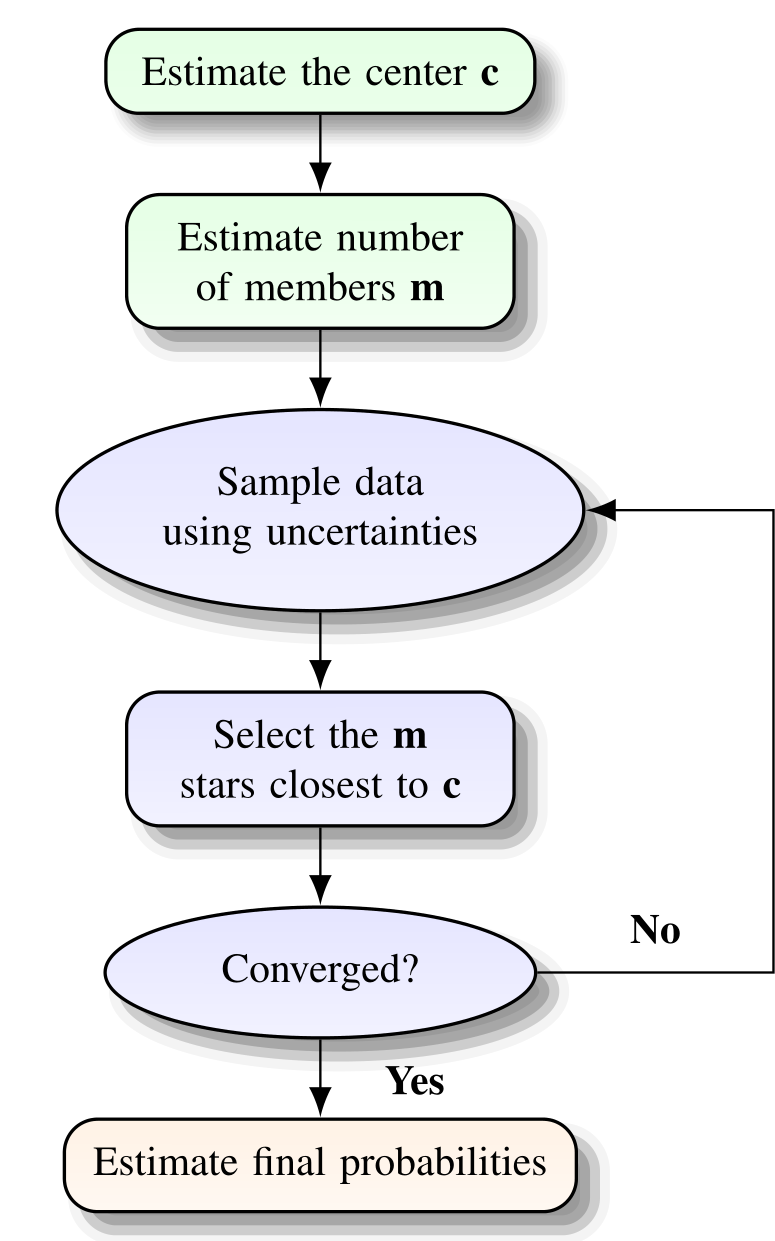
\includegraphics[width=\columnwidth]{figs/flowchart.png}
    \caption{Basic flow chart of the algorithm used by our \texttt{fastMP}
    membership estimation tool.}
    \label{fig:fastMP_code}
\end{figure}


\subsection{Centre estimation}

To determine the most likely centre $c$ for the OC under analysis, the code uses a
three step process. First, it searches for the region of maximum density in
proper motions. Only the 2-dimensional space of proper motions is employed here,
since this is generally where the overdensity is most visible and stands out
against the surrounding contaminating stars in the observed field.
The position of the overdensity is found in an iterative process that starts
with the full set of data, and gradually ``zooms in'' until a convergence
criteria is reached.
The second step selects a subset of stars with the closest distance to this
centre coordinates in proper motions space. In the third step, the final centre
value is obtained using a k-nearest neighbours algorithm to select the point
with the largest density in the 5-dimensional space (coordinates, parallax,
proper motions).


\subsection{Number of members estimation}
\label{ssec:members_estim}

Once centre point is estimated, the total number $m$ of stars that can be
considered members of the OC is obtained through Ripley's K
function~\citep{ripley_1976,ripley_1979}. This function is used to asses how
close a group of points is to a random uniform distribution. We refer the
reader to our previous article where we presented pyUPMASK~\citep{Pera_2021},
where we introduced the concept in much more detail. Subsets of stars are
selected in rings, moving outward from the centre values estimated in proper
motions and parallax. If these stars are considered to be far enough from a
random uniform distribution in coordinates space, they are kept as probable
members of the OC. In this block we can also reject stars that are more
likely to belong to other clusters in the frame, to more accurately estimate the
true number of members for the OC under analysis.

Since it is run only once, Ripley's K function can be replaced by any other
method to estimate the size of a cluster (for example some of the already
mentioned clustering algorithms) without much impact on the performance. It can
even be skipped entirely by feeding this number to \texttt{fastMP}, estimated
manually or by some external process, as explained in the final paragraph of
this section.


\subsection{Sampling, selection, convergence}

This is the bootstrap block where we incorporate the data uncertainties into
the final membership probabilities.
Its basic function is to sample the observed data using its uncertainties,
select those $m$ stars closest to the centre $c$, and
finally repeat this process until a convergence criterion is reached. We define
as a stopping condition the run when the total number of stars with probability
greater than 50\% has stabilized for several of runs.
The bootstrap block is run usually a few hundred times before convergence is
achieved.


\subsection{Membership probabilities}

To estimate the membership probability for each star, the algorithm simply
divides the number of times a given star was selected in the bootstrap block by
the number of runs required until convergence.
In the case where no star was selected by the bootstrap block, probabilities are
assigned based on the 5-dimensional distances to the centre. These are lower
quality probabilities since they do not make use of the uncertainties of the
data. This last resort option is only used for candidate OCs that are either too
faint to be perceptible, or for objects that simply have no detectable stars in a
region of density large enough to be considered stellar clusters.\\


Finally, it is worth noting that an important advantage of \texttt{fastMP} over
tools commonly used like UPMASK, pyUPMASK, HDBSCAN, etc., is that it can run in
supervised mode. In this context, we make the distinction of supervised versus
unsupervised in the sense that the algorithms mentioned above work with no prior
information about the cluster(s) being analysed; we call this ``unsupervised''.
In contrast, \texttt{fastMP} allows information about the cluster to be passed
along with the input data; we call this ``supervised''. Such information can be
the centre of the cluster, its total number of members, or both. If any of these
values are fed to the code after estimating them manually or via an external
method, then its corresponding block (either centre or number of members
estimation)is skipped. This is of great help, particularly
for OCs that are very faint or sparse and can not easily be picked up by the
usual clustering algorithms. It is also a feature that allows the code to
analyse systems that are very close together, either in the positional space
or a combination of this and the proper motions and/or parallax dimensions,
by fixing its centre and/or number of constituent members. In the following
section we show that \texttt{fastMP} has an excellent performance  when compared
to recent works that generate lists of members for OCs, like CANTAT20 and
HUNT23.



%%%%%%%%%%%%%%%%%%%%%%%%%%%%%%%%%%%%%%%%%%%%%%%%%%
\section{Results}
\label{sec:results}

This section is divided as follows. In Sect.~\ref{ssec:duplicates} we analyse
the issue of duplicated entries across catalogues. Sect.~\ref{ssec:members}
compares the results of our membership estimation with those from recent
large catalogues. Sect.~\ref{ssec:classif} discusses a possible
classification of the candidate OCs as real physical objects to separate them
from artefacts derived from the application of different clustering algorithms.
Finally, Sect.\ref{ssec:overview} presents a brief overview of the online
service where this catalogue is hosted and a few of the issues that will be
improved in the future.


\subsection{Duplicates}
\label{ssec:duplicates}

One of the main problems with today's state of research in the area of OCs is,
as mentioned earlier, the large number of articles being published on the subject.
This should not be a concern a priori, but with articles appearing every few
months presenting new candidates by the thousands, keeping track of the
latest proposed objects becomes a not so simple task.
This is evidenced by the large number of potential duplications that can be
found when cross-matching the most recent databases with older ones.

In this work we do not attempt to merge and/or discard candidates as duplicates,
as this is not a trivial assessment to make. The UCC only flags OCs that have
the potential of being duplicates of others, following a parallax-based
decision rule. This rule checks the distance from a given OC to all the others
in the catalogue in three separate components: coordinates (arcmin), parallax 
(mas), and proper motions (mas yr$^{-1}$). If these distances are smaller than a
given threshold, they are converted into a probability using a linear relation;
else they are assigned a probability of zero.\footnote{If the distances in all
three components between the OC and another object are zero, then the
probability of these two being duplicates of each other is 1. If all three
distances are beyond the maximum limits shown in the parallax-based rules, then
the probability of duplication is zero. Distance values beyond zero and these
limits are converted linearly in the probability range (0, 1).}
The relations depend on the distance to the OC (estimated
from its catalogued parallax) and can be seen in the block below.

\begin{verbatim}
if parallax >= 4
    xy_r, plx_r, pm_r = 20, 0.5, 1
else 3 <= parallax < 4
    xy_r, plx_r, pm_r = 15, 0.25, 0.75
else 2 <= parallax < 3
    xy_r, plx_r, pm_r = 10, 0.2, 0.5
else 1.5 <= parallax < 2
    xy_r, plx_r, pm_r = 7.5, 0.15, 0.35
else 1 <= parallax < 1.5
    xy_r, plx_r, pm_r = 5, 0.1, 0.25
else .5 <= parallax < 1
    xy_r, plx_r, pm_r = 2.5, 0.075, 0.2
else parallax < .5
    xy_r, plx_r, pm_r = 2, 0.05, 0.15
else parallax < .25
    xy_r, plx_r, pm_r = 1.5, 0.025, 0.1
else parallax is nan
    xy_r, pm_r = 2.5, 0.2
\end{verbatim}

Here, \texttt{xy\_r, plx\_r} and \texttt{pm\_r} are the parallax-based
thresholds for each component (in arcmin, mas, and mas yr$^{-1}$; respectively).
For example, if a candidate OC has a catalogued parallax of 0.75 mas, then 
\texttt{xy\_r, plx\_r, pm\_r = 2.5, 0.075, 0.2}. This
means that any other OC with distances smaller than those thresholds in any (or
all) of the components, will have a non zero probability of being a duplicate;
where a larger probability is associated to smaller distances.
The reason to split the threshold in parallax ranges is that the farther away
the OC the smaller its parallax, coordinates radius, and mean proper motions
will tend to be. These thresholds and parallax ranges are of course entirely
arbitrary, but we have observed very reasonable results using them.
%
Employing this rule, the aforementioned OC candidate CWDDL 14677 is flagged with
a 65\% probability of being a duplicate of Blanco 1; if the catalogued positions
are used. If we use the values for the main coordinates, proper motions, and
parallax obtained from the most likely members found by \texttt{fastMP}, this
probability increases to 84\%.\\

\begin{figure}
	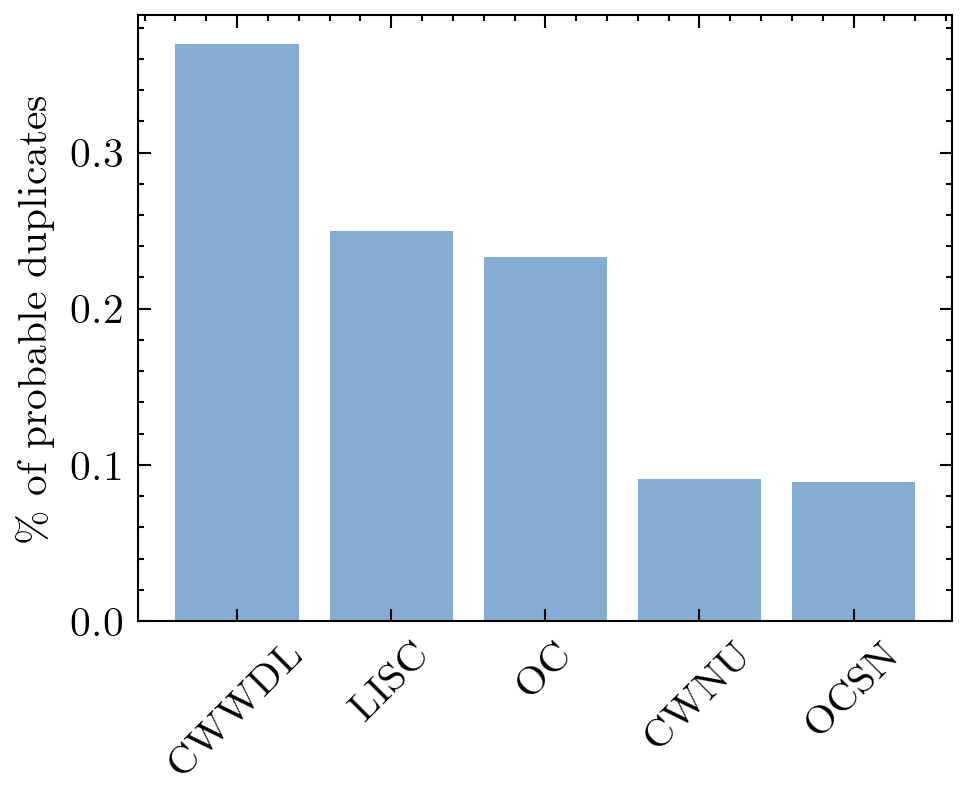
\includegraphics[width=\columnwidth]{figs/duplicates.png}
    \caption{Percentage of probable duplicates for five recent databases of
    candidate OCs presented in the literature, characterized by their IDs.
    See Table~\ref{tab:references} to match the corresponding article(s)
    to each ID.}
    \label{fig:duplicates}
\end{figure}

In Fig.~\ref{fig:duplicates} we show the percentage of entries flagged as
probable duplicates for five of the latest articles mentioned in
Table~\ref{tab:references}. We selected as probable duplicates those entries
with an assigned probability larger than 50\%.
The CWWDL clusters from~\cite{Chi_2023_3} stand out with almost 40\% of its
1179 candidate OCs flagged as probable duplicates of entries in previous (older)
catalogues. This is a rather large value that translates to more than 400 of the
candidate OCs listed in this catalogue.

An example of two candidate OCs flagged as possible duplicates, with a
probability value of 50\% and 90\%, are CWWDL 578~\cite{Chi_2023_3} and
LISC 3279~\citep{Li_2022}. These objects
were associated by our parallax-based rule to two UBC OCs, presented
in~\cite{Castro-Ginard_2020}.
The five dimensional positions catalogued values for these four entries
are shown in Table~\ref{tab:duplicates}.
% At first glance, these look very much like the same object listed twice.
Although we understand that such a simple rule based on distances in the
coordinates, parallax, and proper motion spaces is not a replacement for a
proper detailed analysis on duplication, it can certainly serve as a reasonable
starting point. Studies on systems of binary clusters can base their initial
assessment on these probabilities as well. There are in total more than 2000
entries in the UUC flagged as being a duplicate, or flagged as having one or
more duplicates, which amount to $\approx$15\% of the entire catalogue.

\begin{table}
	\centering
	\caption{Examples of two pairs of OCs flagged as duplicates by our
	parallax-based rule with probabilities of 50\% (1st and 2nd columns) and
	90\% (3rd and 4th columns).}
	\label{tab:duplicates}
	\begin{tabular}{lcccc}
		\hline
         &  \multicolumn{2}{c}{P$\approx$50\%} & \multicolumn{2}{c}
         {P$\approx$90\%}\\
          &   CWDDL 578 & UBC 395 & LISC 3279  &  UBC 361 \\
		\hline
		 RA &   345.743 & 345.655 & 290.000  &  290.016 \\
		 DEC &   57.231 & 57.206 & 15.146  &  15.157 \\
		 Plx &   0.412 & 0.409 & 0.630  & 0.632 \\
		 pmRA &   -2.844 & -2.869 & -1.669  & -1.701 \\
		 pmDE &   -2.542 & -2.591 & -5.225  & -5.232 \\
		\hline
	\end{tabular}
\end{table}



\subsection{Membership analysis}
\label{ssec:members}

More than one million estimated members are stored in this initial version of
the UCC; this is almost half a million more than those in the HUNT23 catalogue 
(after removing globular cluster and moving groups), and approximately five
times those in CANTAT20. This last database is expected to contain
less entries not only because it is smaller regarding the number of OCs listed,
but also because it only reaches G=18 mag, whereas UCC and HUNT23 go two
magnitudes further down.

In the top plot of Fig.~\ref{fig:members} we show the distribution of
estimated members for these three catalogues versus Gaia's G magnitude. The
centre plot shows the same distributions but normalized by the total number of
entries in each catalogue. Finally, the bottom plot shows the percentage of
members in CANTAT20 and HUNT23 matched to members estimated by the UCC. While
CANTAT20 displays an overall match in the range $\sim$75-80\% for the entire
magnitude span, up to its maximum of G=18 mag, the match with HUNT23
hovers around 70-75\% up to G$\approx$17 mag after which it begins to drop.
For the largest magnitude in UCC and HUNT23, G=20 mag, the match
percentage is $\sim$35\%. This can be explained mainly by two processes.
%
In one hand, the large sensitivity of the HDBSCAN algorithm often causes it to
return false positives, as reported by HUNT23. This can translate to
an overconfidence in the number of members assigned to each candidate OC.
On the other hand, the methods employed in CANTAT20 and HUNT23, UPMASK and
HDBSCAN respectively, do not make use of the uncertainties of Gaia's data
whereas \texttt{fastMP} does. Incorporating uncertainties into the membership
probabilities estimation affects stars in the lower mass region the most, as
these are the ones with the largest errors. The \texttt{fastMP} code also uses a
more cautious approach when estimating the total number of stars associated to a
given OC, based on Ripley's K function as mentioned in
Sect.~\ref{ssec:members_estim}. The centre plot in Fig.~\ref{fig:members}
clearly shows these effects, where normalizing by the number of OCs in each
catalogue makes the UCC's distribution dip below those of CANTAT20 and HUNT23.
The UCC has a combined $\sim$90 members per OC, HUNT23 has around $\sim$110
members per OC, and CANTAT20 is close to $\sim$95 members per OC.
%
% Given that CANTAT20 only includes stars up to G=18 mag one would expect
% the number of average members per OC to be at least $\sim$20\% lower than those
% of HUNT23 or the UCC; this is $\sim$80 members per OC. 

% Fig members vs HUNT23 and CANTAT20
\begin{figure}
	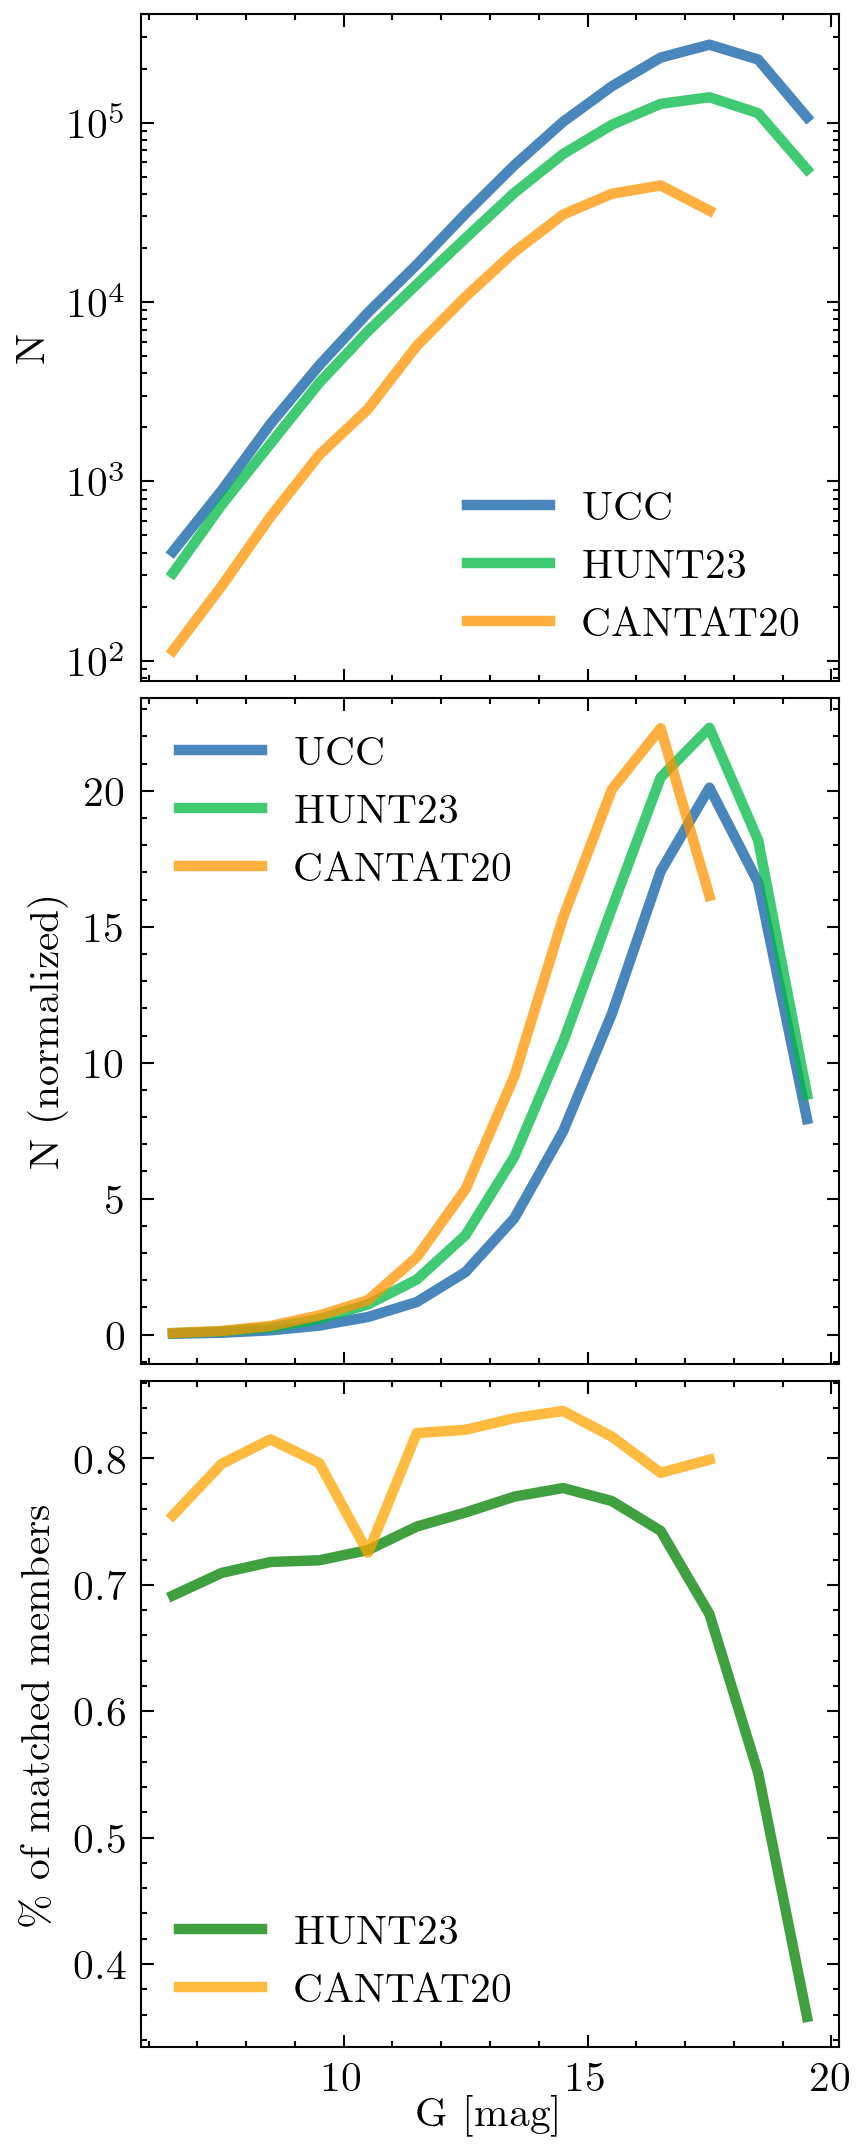
\includegraphics[width=\columnwidth]{figs/membs_compare.png}
    \caption{Top: total number of identified members versus magnitude, for
    the catalogues HUNT23, CANTAT20, and the UCC.
    Center: same as above but normalized by the total number of entries in each
    catalogue.
    Bottom: percentage of members in HUNT23 and CANTAT20 matched with members
    identified by the UCC, versus magnitude.}
    \label{fig:members}
\end{figure}

% A particular case where this effect is markedly visible is OC NGC 6167. Our
% \texttt{fastMP} method estimates almost 600 members while HUNT23 estimates more
% than 2500. A manual analysis results in an estimation of $\sim$1500 members for
% this OC, i.e. approximately the middle point between both estimates. An
% advantage of \texttt{fastMP} is that it can also work in supervised mode, which
% means we can fix the approximate number of members to the manually estimated
% value. We show in Fig.~\ref{fig:ngc6167} the results of these three processes.

% % NGC 6167 vs HUNT23 vs manual
% \begin{figure*}
% 	\includegraphics[width=\textwidth]{figs/ngc6167.png}
%     \caption{Analysis of the OC NGC 6167 by HUNT23 (green), \texttt{fastMP}
%     under supervised mode with fixed number of members at 1500 (cyan), and 
%     \texttt{fastMP} under unsupervised mode (blue).}
%     \label{fig:ngc6167}
% \end{figure*}



\subsection{Classification}
\label{ssec:classif}

Determining what constitutes a true physical cluster of stars is not an easy
task when dealing with OCs. Whereas globular clusters are made of hundreds of
thousands of member stars, OCs are much smaller. In the previous section we
showed that, for the three largest catalogues published recently including
the UCC, a reasonable general average for the number of members in an
OC is of the order of just 100 stars; with a heavy skew towards smaller values.
A proper physical analysis of whether a few dozen stars are gravitationally
bound requires information that we currently lack, particularly the individual
masses (or a reliable total mass estimation) and precise velocities.

% Fig Plx vs PMs distribution, UCC vs HUNT23 vs CANTAT20
\begin{figure*}
	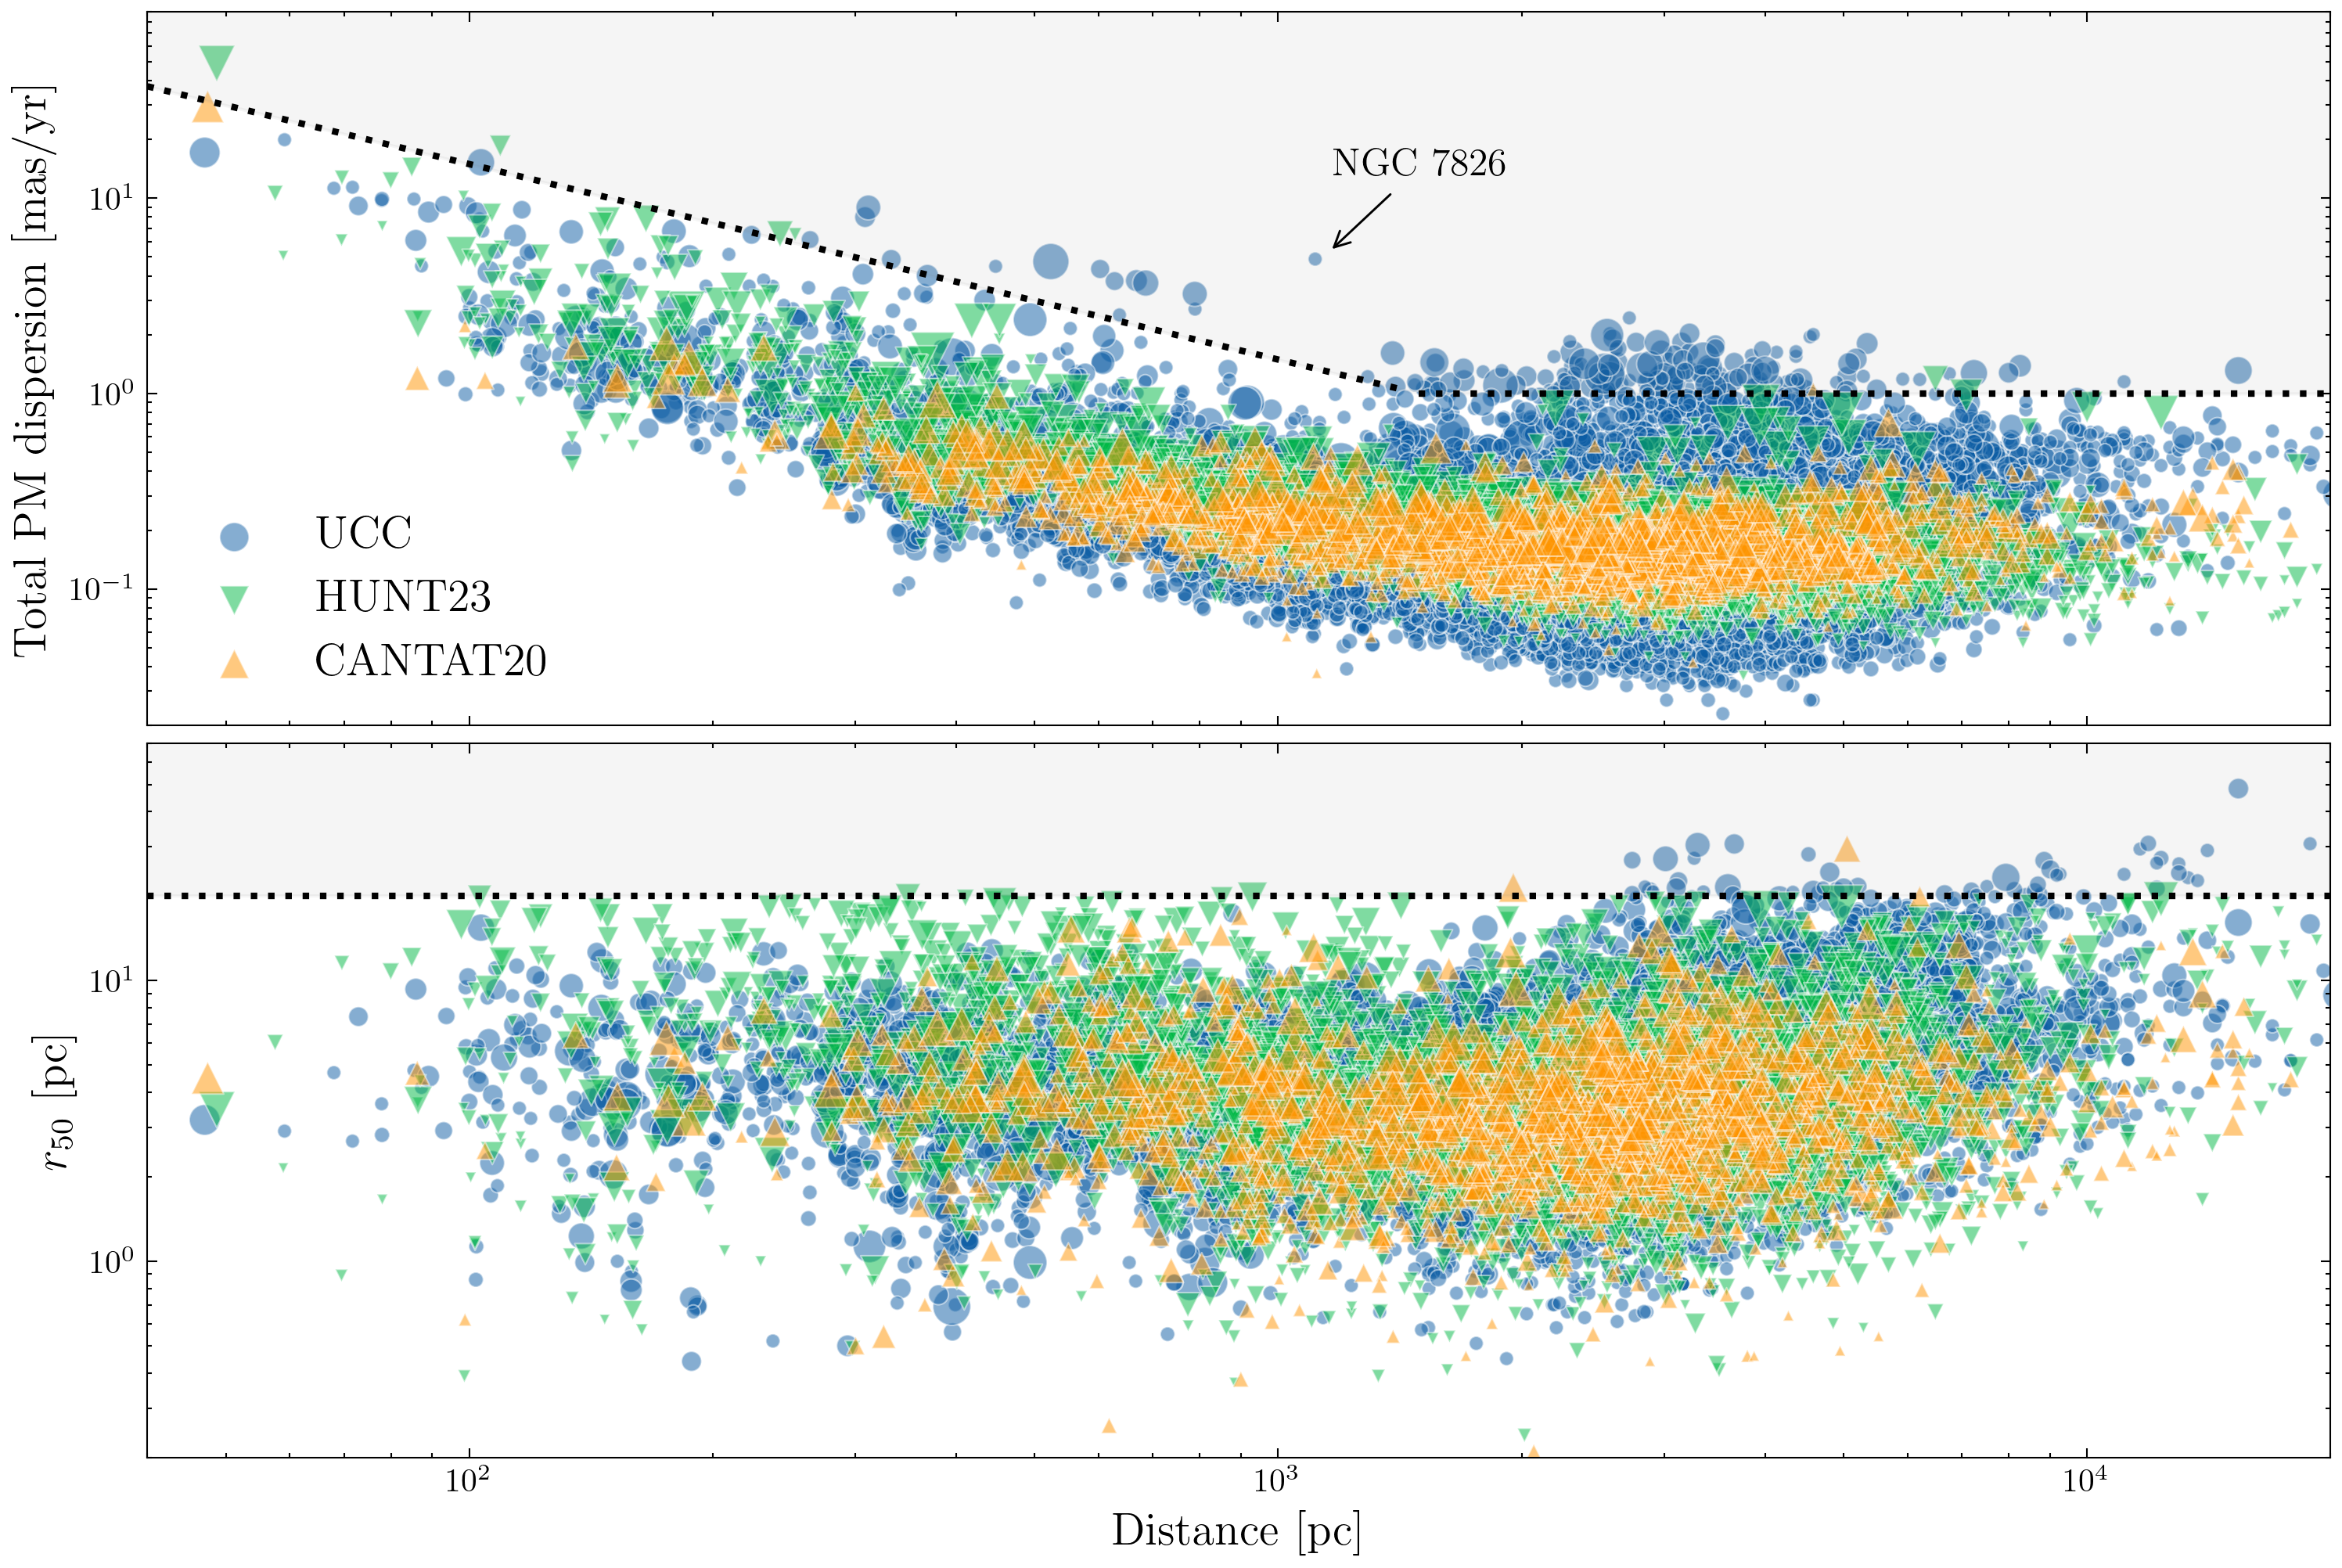
\includegraphics[width=\textwidth]{figs/pms_plx.png}
    \caption{Distribution of total proper motion dispersion (top) and radius
    that contains half the members (bottom) versus distance, for the candidate
    OCs listed in CANTAT20 (orange), HUNT23 (green), and the UCC (blue).
    Sizes are proportional to each candidate's associated number of members.
    The grey region in both plots is the ``not true OC region'' defined by
    the rules proposed by \citet{Cantat-Anders_2020}.}
    \label{fig:pms_plx}
\end{figure*}

This fact notwithstanding, there are still methods we can use to approximate
a full dynamical analysis to characterize candidate OCs as more or less likely
to be real. Two of these methods, or quality cuts, were proposed
by~\cite{Cantat-Anders_2020}.
The first one is based on the fact that we can set an upper limit to the
internal velocity dispersion of OCs, beyond which objects should either be
globular clusters or unbound groups. Conservatively, this limit is 5
km\,s$^{-1}$, but it is relaxed to 1 mas\,yr$^{-1}$ for candidate OCs
beyond $\sim$1000 pc for which uncertainties in the proper motions tend to
dominate the measured values.
We set the break between both limits at $\sim$1.5 kpc, the distance
where the velocity dispersion lines mentioned above intersect.
%
The second method is a measure of the internal spatial dispersion of an OC.
In~\cite{Cantat-Anders_2020} it is stated that, for the majority of
bonafide OCs, the maximum dimension that contains half the members can be set to
$\sim$15 pc; HUNT23 relaxes this condition slightly to 20 pc, which we also
adopt.
In Fig.~\ref{fig:pms_plx} we show the result of both these approaches to
approximate a ``true OC region'' on the data collected in the UCC, along with
that presented in CANTAT20 and HUNT23.
As can be seen, the region occupied for the three catalogues is very similar
with the UCC showing a broader distribution in total proper motions dispersion
beyond $\sim$1000 pc.
Nonetheless, the large majority of candidate OCs are well below the proposed
cuts in both plots. Those objects with large proper motion dispersions are
mostly candidates listed only in the~\cite{Kharchenko_2012} catalogue that were,
to the best of our knowledge, never properly analysed. There are also $\sim$30
OCs from~\cite{Ryu_2018} (infrared candidates) whose membership estimation
is poor.

An example of an object that is located beyond the proper motions dispersion
quality cut is NGC 7826, identified in the top plot of Fig.~\ref{fig:pms_plx}.
This object has been discarded as a true OC in~\cite{Kos_2018} and listed as an
asterism in~\cite{Cantat-Anders_2020}, but we include it nonetheless as it is
listed in the~\cite{Loktin_2017} catalogue. Expectedly, the proper motions
distribution of its most likely associated stars also exclude it from the
``true OC region'' in this work.\\

We can also define other metrics to classify candidate OCs into more or less
likely true physical objects, employing their estimated members' data. The first
metric we developed is a density-based classification, $C_{dens}$, and the
second one is a photometry-based classification, $C_{phot}$.
These are similar in conception to the CST score and CMD class defined in
HUNT23, respectively.
The density-based metric compares the distribution of member stars to the
distribution of close-by field stars, in the 5-dimensional space of coordinates,
proper motions and parallax. The reasonable expectation is that neighbouring
cluster members should have smaller average distances than neighbouring field
stars.
The photometry data is processed separately because member stars of an OC in a
colour-magnitude diagram (CMD) do not cluster together around a centre value, as
they do in the remaining data dimensions. Instead, they are distributed
following an elongated path across the evolutionary sequence. For this reason we
do not employ a closest-neighbour density based method, but one based on the
likelihood of the members' sequence of being equivalent to a random sequence
drawn from field stars. To quantify this we make use of the same function
written for our \texttt{ASteCA} package~\citep{Perren_2015}, based on the
Poissonian distribution likelihood defined in~\cite{Tremmel_2013}.
Fig~\ref{fig:classification} shows the distribution of these two metrics, both
normalized in the [0, 1] range where 1 means most likely to be a collection
of related cluster member stars in either metric. The colour is assigned
according to the vertical distance to the quality cut in the total proper
motions dispersion diagram shown in the top plot of Fig.~\ref{fig:pms_plx}.
Objects that are beyond these limit (i.e., larger proper motions
dispersion than that allowed for an OC) have values below zero and are drawn
in purple. Sizes follow the spatial extension of the estimated members.
A clear tendency can be seen where candidate OCs with larger $C_{dens}$ values
also display large $C_{phot}$ values, which is expected. There is also a visible
scatter around the 1:1 identity relation, meaning these two metrics are not
entirely correlated. This is desirable, otherwise both methods would be
returning the same information. Objects with large total proper motion
dispersions are mostly correlated with low $C_{dens}$ values but tend to span
the entire range of $C_{phot}$ values.

% Fig classes (lkl, density)
\begin{figure}
	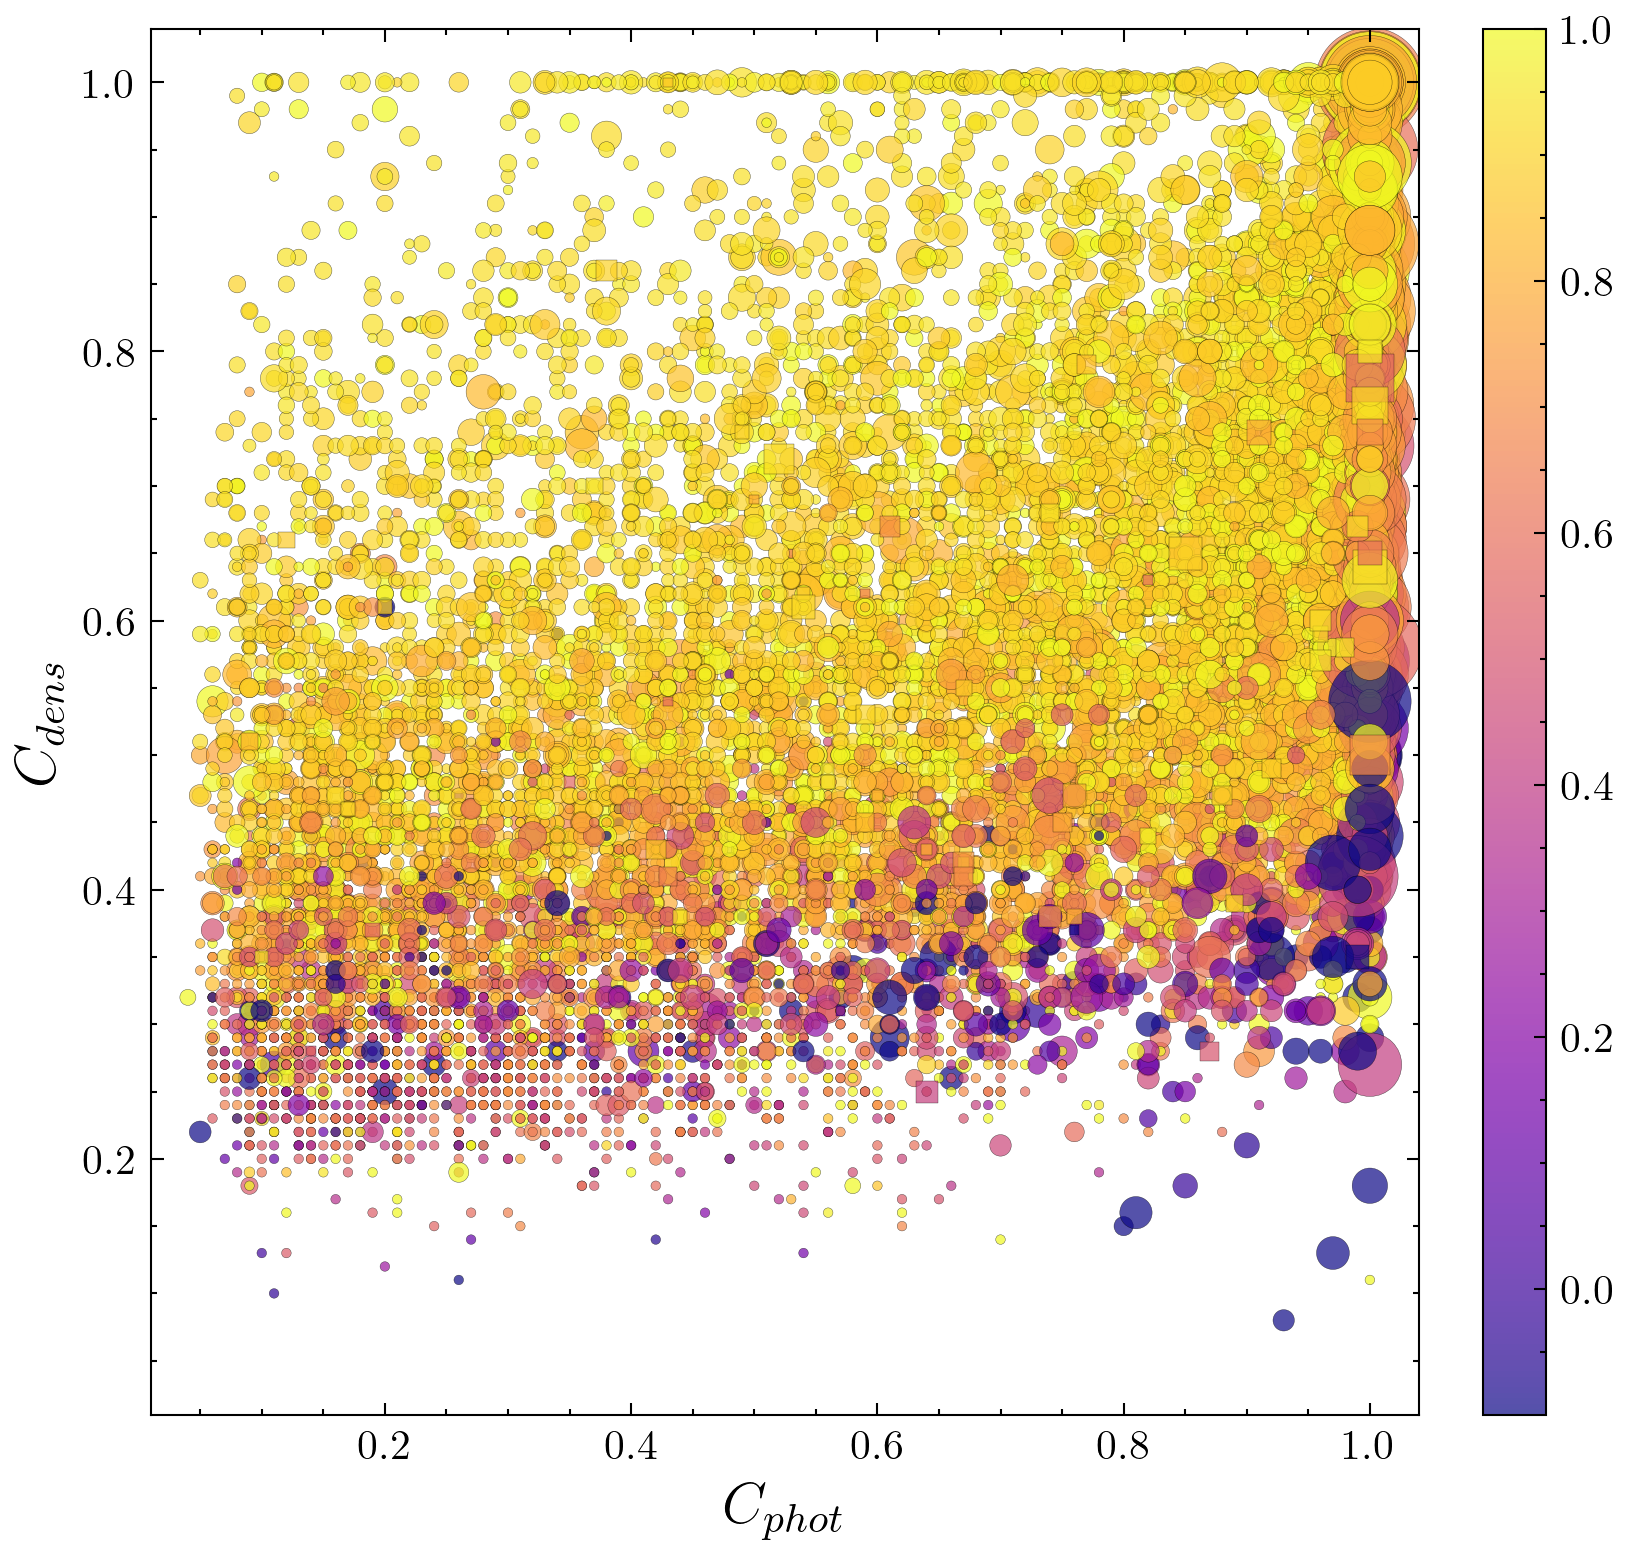
\includegraphics[width=\columnwidth]{figs/classif.png}
    \caption{Five dimensional density $C_{dens}$ versus photometry based metric
    $C_{lkl}$ for the candidate OCs listed in the UCC. Colour is related to the
    vertical distance to the total proper motion quality cut; the colourbar is
    clipped at -0.1 and 1 to improve visibility. Size is related to
    the spatial extension of its members. Squares are
    associated to candidates beyond the 20 pc spatial dispersion quality cut.}
    \label{fig:classification}
\end{figure}

We take these two classification metrics and combine them into a single quality
class for each candidate OC, to provide a quick glance of the characteristics of
the estimated members for the catalogued objects.
First we split the [0, 1] range for both metrics into 4 equal length segments 
(from 0 to 0.25, from 0.25 to 0.5, etc.) and assign a letter to each from D for
the [0, 0.25] segment, to A for the [0.75, 1] segment.
These two letters, one for each metric, are combined to generate a single class
out of 16 possible combinations. The letter that corresponds to the $C_{phot}$ 
value is positioned first, followed by the letter obtained for the $C_{dens}$
value for that object. The better quality clusters are thus assigned AA classes
whereas the lowest quality ones DD classes.
The complete distribution of classes is shown in Fig.~\ref{fig:classif_bar}.
The three better quality classes (AA, AB, and BA), group more than 5300
objects ($\sim$40\% of the catalogue), while the lowest three classes (CD,
DC, and DD) contain almost 2000 candidate OCs or $\sim$15\% of the UCC
catalogue. The classes AD and DA are two of the least populated, meaning that it
is not likely to find an object with a large value in $C_{phot}$ and a low value
in $C_{dens}$ or vice versa; as one would expect.

\begin{figure}
	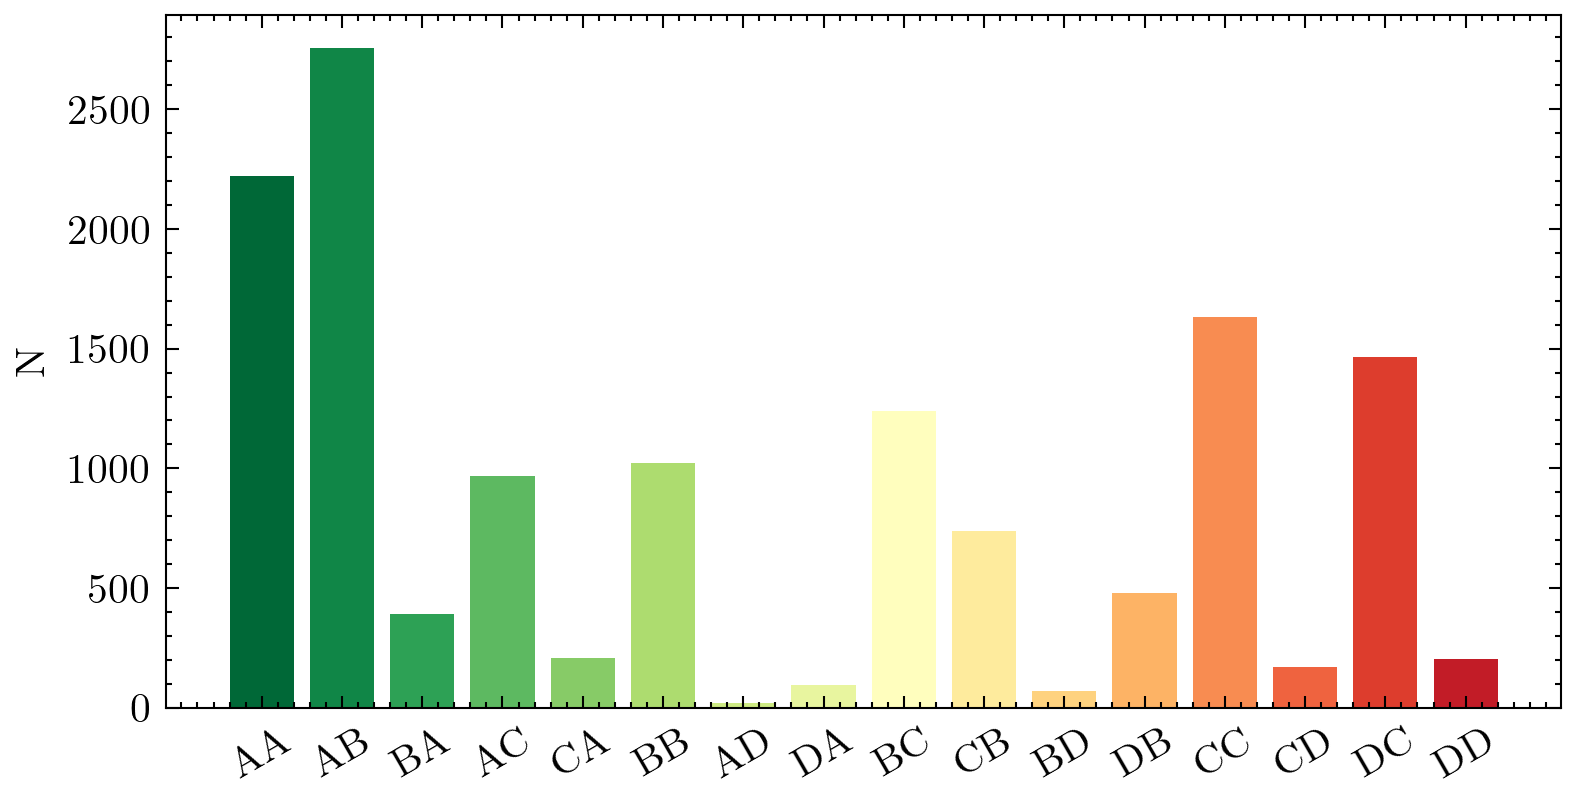
\includegraphics[width=\columnwidth]{figs/classif_bar.png}
    \caption{Distribution of the quality classes obtained combining the
    $C_{phot}$ and $C_{dens}$ values for each OC as described in the text.}
    \label{fig:classif_bar}
\end{figure}

In Fig.~\ref{fig:classif_examples} we show examples of four OCs listed in the
UCC with combined classes of AA, BB, CC, and DD. The difference is clear between
the better AA and worse DD classes, both in the more dense spatial, proper
motions, and parallax distributions; as well as the sharper definition of the
cluster sequence in the CMD.\\

\begin{figure*}
	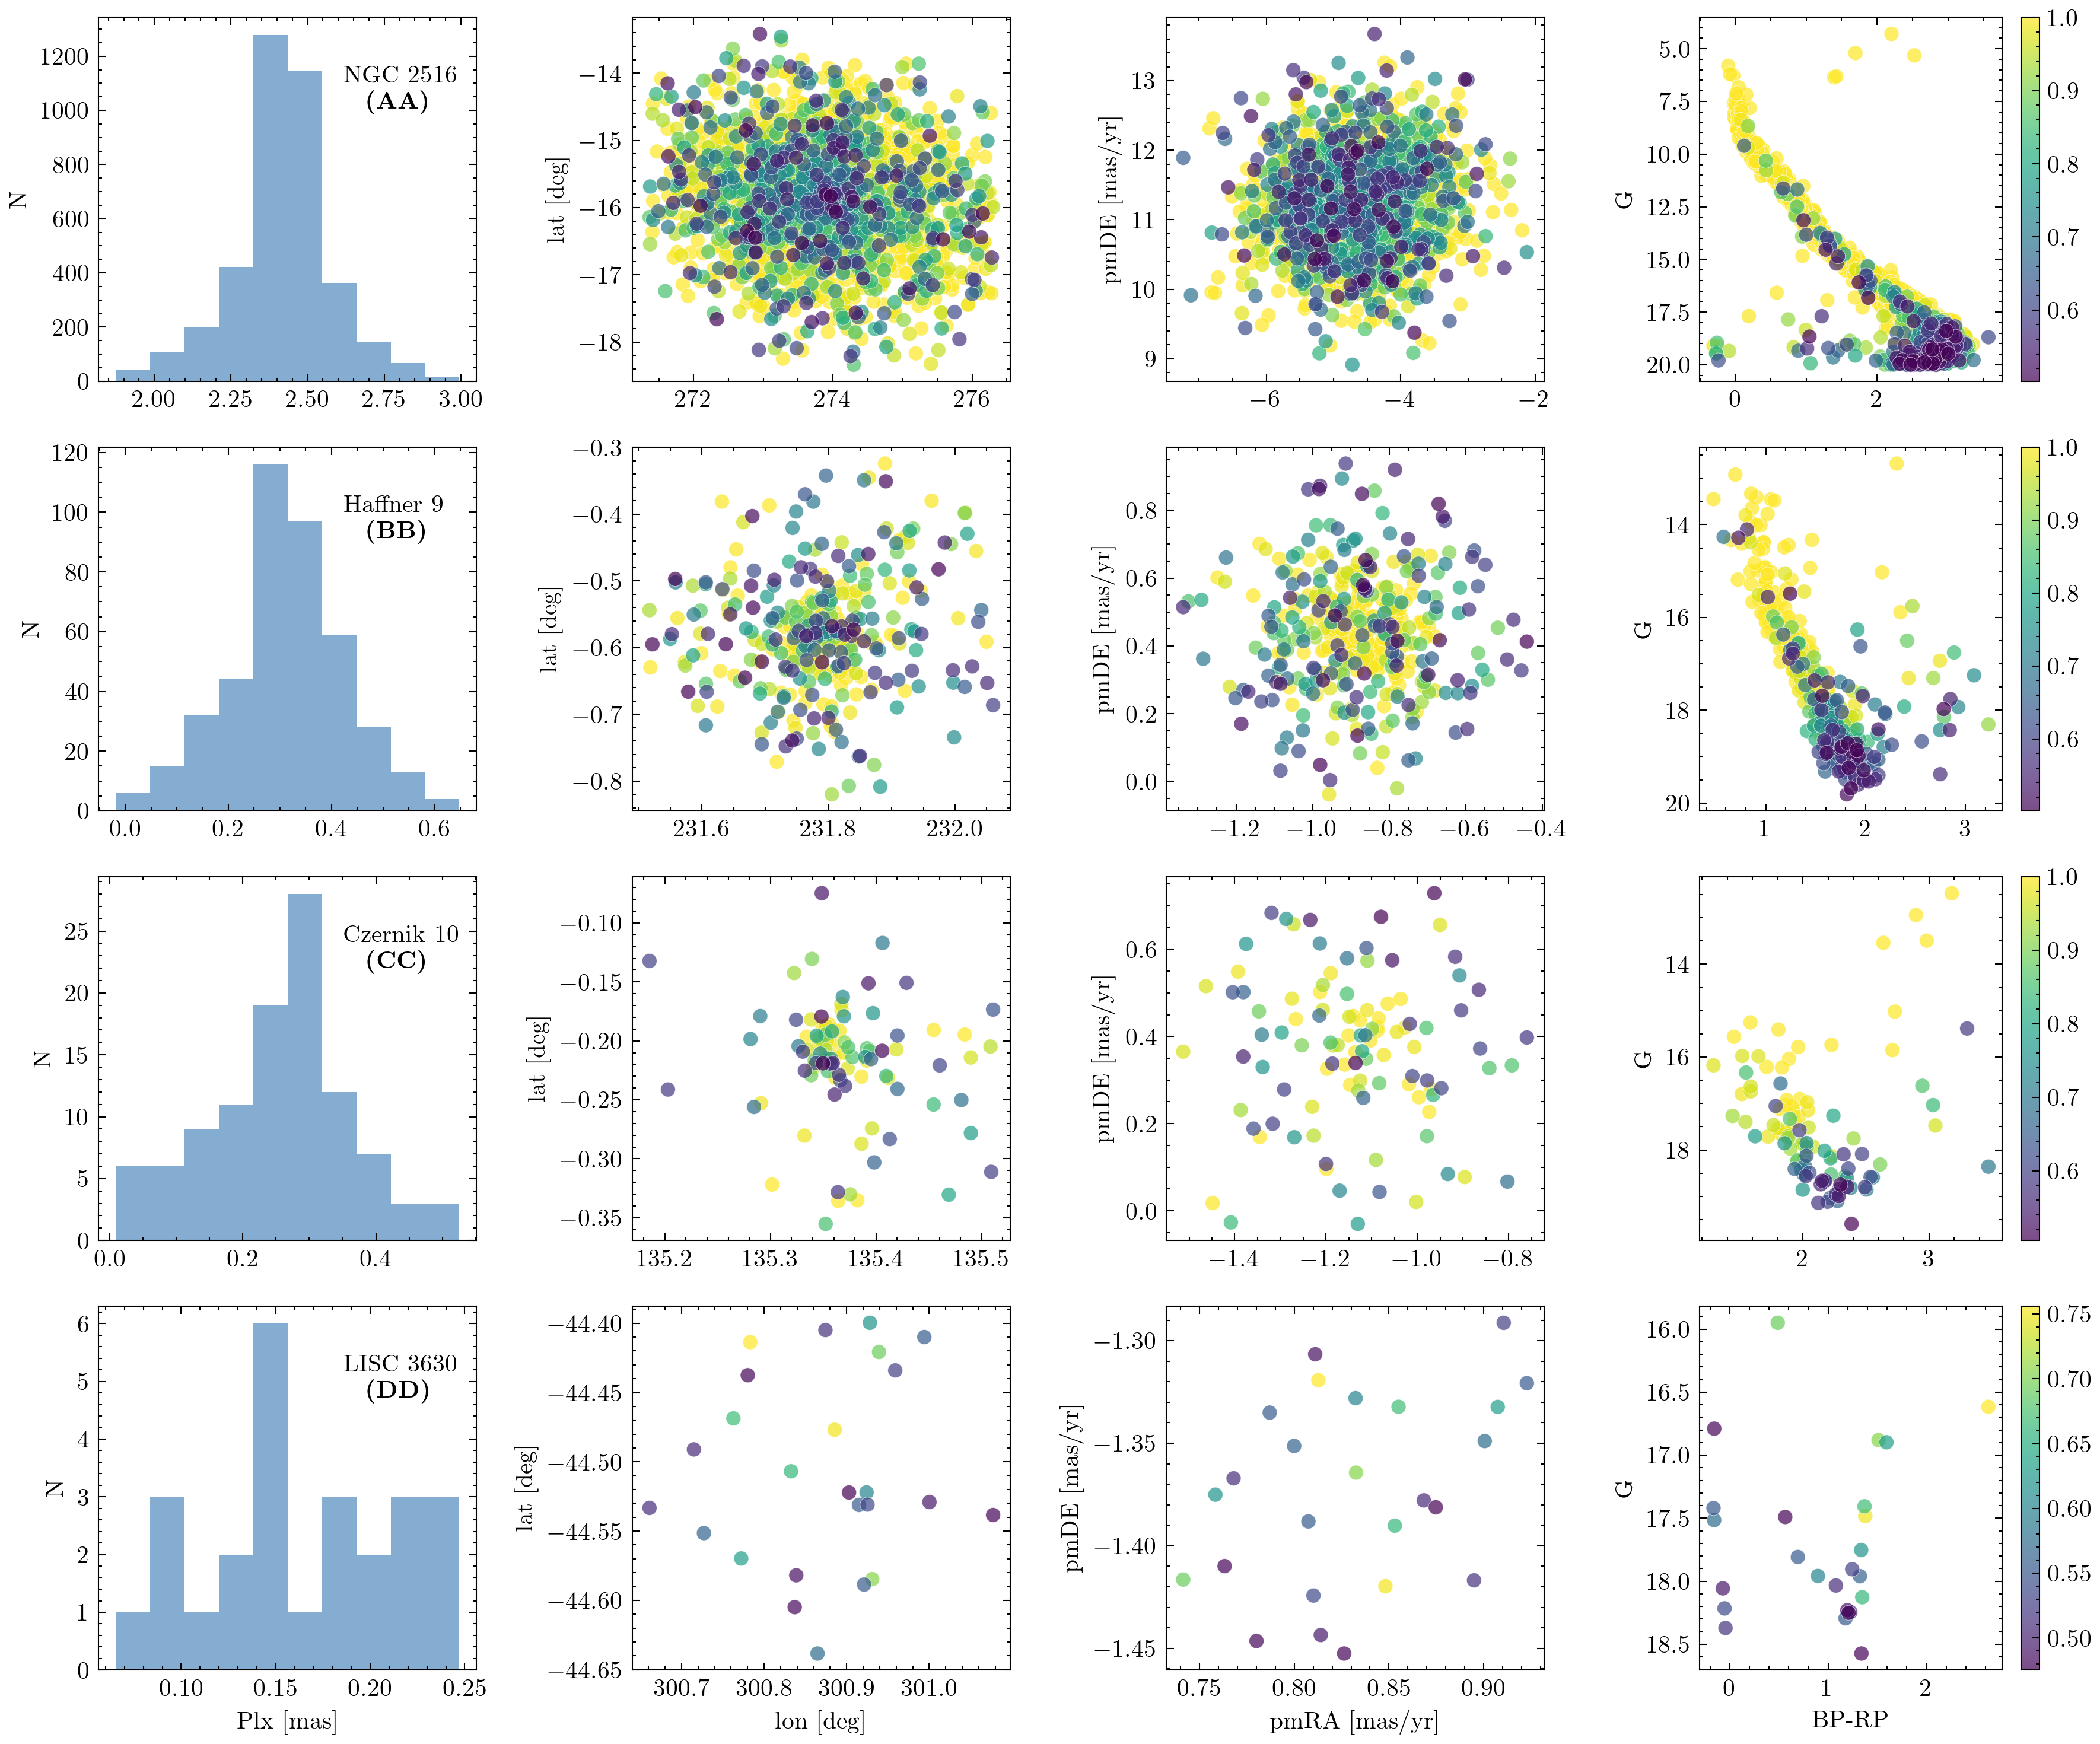
\includegraphics[width=\textwidth]{figs/clusters_classif.png}
    \caption{Examples of listed OCs with combined classes AA, BB, CC, and
    DD from top to bottom rows, respectively. Plots show from left to right:
    parallax distribution, spatial dispersion, proper motions, and CMD;
    respectively.
    Colourbars are associated to the membership probabilities assigned by 
    \texttt{fastMP}.}
    \label{fig:classif_examples}
\end{figure*}

These quality cuts and classification methods are unfortunately not
enough to completely replace a proper analysis of a candidate OC. We can of
course use them as guides to identify problematic cases, but their values still
depend heavily on the precision of the membership estimation process. If this
process did a poor job, which it will undoubtedly do for the more complicated
cases, then these results will be compromised.
More and better quality for the data of observed stars will hopefully improve
this scenario in the near future.






\subsection{Overview of the service}
\label{ssec:overview}

To facilitate cross-catalogues identification of entries, each candidate OC in
the UCC is assigned a unique name following the International Astronomical
Union's specifications. The naming convention is formatted as \emph{UCC
GLLL.LsBB.B}; where \emph{UCC} is the catalogue's name, \emph{G} indicates that
we are using galactic coordinates, \emph{LLL.L} is the (truncated) longitude
for the object, \emph{s} is the sign of its latitude, and \emph{BB.B} is the 
(truncated) latitude. If two objects share coordinates, a lowercase letter from
a to z is added to the end of the name.

%
The spatial position of each entry in the catalogue is displayed making use of
Aladin's visualization tool,\footnote{Aladin: 
\url{http://aladin.cds.unistra.fr/}}
showing the coordinates, proper motions, parallax, and radial velocity values
associated to it, when present from the literature.
Links to search the cluster's main name in the SAO/NASA Astrophysics Data System
(ADS)\footnote{SAO/NASA ADS: \url{https://ui.adsabs.harvard.edu/}} as well as
a region search in the Strasbourg astronomical Data Center
(CDS)\footnote{CDS: \url{http://cdsportal.u-strasbg.fr/}} are provided. A Python
notebook hosted in Google's Colaboratory
service\footnote{Colaboratory: \url{https://colab.research.google.com/}} is made
available, to allow the user interactive exploration of the Gaia survey data of
each candidate's estimated members. In this initial version the UCC only
contains membership data obtained through our own \texttt{fastMP} tool. In
future updates we will add the members estimated by other works, such as those
from CANTAT20 and HUNT23, as well as the most recent catalogues.

Fundamental parameters such as distance, extinction, age, and metallicity are
also shown when available, taken from as many databases as possible. This will
also be expanded in future updates of the UCC, as more values from the
literature are incorporated. For each candidate OC its nearby entries and
possible duplicates are also shown, along with the probability of being a
duplicate obtained as detailed in Sect.~\ref{ssec:duplicates}.

In an upcoming version of the UCC we will add individual notes whenever
available. These are much more difficult to acquire as they tend
to be scattered throughout the literature instead of compiled in databases.
For example~\cite{Cantat-Anders_2020} contains in its appendix a list of OCs
classified as asterisms; information that is lost if only the parameters of
the candidate are displayed in the catalogue.





% Collinder_393 & Collinder_394: HUNT23 merges both as one (Collinder 394 is
% mentioned in the article)
% NGC_2184, Collinder_107, VFBH_205: wrong cluster in HUNT23
% UBC_517, Ruprecht_163: very extended, fastMP does not find overdensity
% Ruprecht_123: wrong members because of DIAS21 bad PMs
% UBC1_541: bad PM center in fastMP
% these values are correct)
% Waterloo_1: HUNT23 appears to append a second non-catalogued OC
% Bochum_1: LOKTIN17 slightly wrong RA, binary cluster?
% Trumpler_24: very extended in frame
% UBC_186: CANTAT20 selects NGC 581
% HSC_46: fastMP detects the 'tail' of GC NHC 5904 with plx=0.14 and assigns
% many more stars than HUNT23





%%%%%%%%%%%%%%%%%%%%%%%%%%%%%%%%%%%%%%%%%%%%%%%%%%
\section{Conclusions}
\label{sec:conclusions}

We presented the Unified Cluster Catalogue or UCC, along with its accompanying
tool for membership probabilities estimation, the \texttt{fastMP} code. This is
the largest catalogue of open clusters to date and it will be regularly updated
as new databases are made public in the literature. The UCC is accessible
through its own dedicated web site at \url{https://ucc.ar} where each OC is
displayed along with its fundamental parameters (gathered from the literature
when available), allowing the user to interactively explore the data online
through Python notebooks hosted by the Google Colaboratory service. In its
initial version the UCC lists almost 14000 unique candidate OCs whit a combined
number of proposed homogeneously obtained member stars larger than 1 million,
or $\sim$90 member stars per OC.

Replacing the trained eye of a researcher even for the initial assessment
of what constitutes a true OC in a completely generalized approach, is no
easy task. With new candidate OCs being presented in the literature by the
hundredths or thousands every few months, a systematic method for addressing
this issue becomes more and more pressing.
Our classification parameters were created to help with this task, but a close
visual inspection is still required; particularly for the more complicated
objects.
We expect the Unified Custer Catalogue and its associated online service to be a
useful resource for the astrophysical research community, and welcome all
suggestions to expand and/or improve it in the future.



%%%%%%%%%%%%%%%%%%%%%%%%%%%%%%%%%%%%%%%%%%%%%%%%%%
\section*{Acknowledgements}

The authors would like to thank Dr Emily Hunt for her assistance with the
processing of the HUNT23 database.
%
This work has made use of data from the European Space Agency (ESA) mission
{\it Gaia} (\url{https://www.cosmos.esa.int/gaia}), processed by the {\it Gaia}
Data Processing and Analysis Consortium (DPAC,
\url{https://www.cosmos.esa.int/web/gaia/dpac/consortium}). Funding for the DPAC
has been provided by national institutions, in particular the institutions
participating in the {\it Gaia} Multilateral Agreement.
%
This research has made use of the WEBDA database, operated at the Department of
Theoretical Physics and Astrophysics of the Masaryk University.
%
This research has made use of the VizieR catalog access tool, operated at CDS,
Strasbourg, France~\citep{Ochsenbein_2000}.
%
This research has made use of ``Aladin sky atlas'' developed at
CDS, Strasbourg Observatory, France~\citep{Bonnarel2000,Boch2014,Baumann_2022}.
%
This research has made use of NASA's Astrophysics Data System.
%
This research made use of the Python language~\citep{vanRossum_1995}
and the following packages:
NumPy\footnote{\url{http://www.numpy.org/}}~\citep{vanDerWalt_2011};
SciPy\footnote{\url{http://www.scipy.org/}}~\citep{Jones_2001};
matplotlib\footnote{\url{http://matplotlib.org/}}~\citep{hunter_2007};
scikit-learn\footnote{\url{https://scikit-learn.org/}}~\citep{scikit-learn};
\texttt{ASteCA}\footnote{\url{https://github.com/asteca}}~\citep{Perren_2015}.
%
This work made use of Astropy:\footnote{\url{http://www.astropy.org}} a
community-developed core Python package and an ecosystem of tools and resources
for astronomy \citep{astropy:2013, astropy:2018, astropy:2022}.





%%%%%%%%%%%%%%%%%%%%%%%%%%%%%%%%%%%%%%%%%%%%%%%%%%
\section*{Data Availability}
 
The data underlying this article are available in the repositories associated to
the Unified Cluster Catalogue, accessible at \url{https://github.com/ucc23}.
The code employed to process the data and generate the images in this article
con be found in the repositories for the \texttt{fastMP} code at 
\url{https://github.com/Gabriel-p/fastMP}, and in the repository for the article
itself at \url{https://github.com/gabriel-p-artcls/GDR3_members}. Any missing
data file and/or code file can be requested to the corresponding author and we
will gladly make it available.




%%%%%%%%%%%%%%%%%%%% REFERENCES %%%%%%%%%%%%%%%%%%

% The best way to enter references is to use BibTeX:

\bibliographystyle{mnras}
\bibliography{biblio} % if your bibtex file is called example.bib


%%%%%%%%%%%%%%%%%%%%%%%%%%%%%%%%%%%%%%%%%%%%%%%%%%



%%%%%%%%%%%%%%%%% APPENDICES %%%%%%%%%%%%%%%%%%%%%

\appendix

\section{Databases cleaning}
\label{app:db_cleaning}

We describe here a summary of the cleaning and standardizing processes applied
on almost all of the catalogues mentioned in Table~\ref{tab:references}. Most of
these are small tasks, like manually editing names so that they are
consistent across databases, but they were necessary (and rather time
consuming). For convenience we abbreviate \cite{Kharchenko_2012} as KHAR12 and
\cite{Bica_2019} as BICA19.
The catalogue used for identifying globular clusters (GCs) is that
of~\cite{Vasiliev_2021} with the addition of the Gran 2, 3, 4, and 5 objects
from~\cite{Gran_2022}.\\

\noindent\cite{Kharchenko_2012}: Selected all entries with \emph{class} equal to
``OPEN STAR CLUSTER'', resulting in 2858 entries. The astrometry values in this
database are of low quality, we do not use these values in the
membership estimation process.
Added the preferred denomination VDBH to vdBergh-Hagen and VDB to vdBergh
clusters, per CDS recommendation (this is done across all the catalogues).
Removed entries that match galactic clusters: ESO 456-29 (Gran 1), FSR 1716,
FSR 1758, VDBH 140.\\

\noindent\cite{Loktin_2017}: Many proper motion values in this catalogue are clearly
wrong (e.g: the values for NGC 2516). We thus do not use these values in the
membership estimation process.
Removed entries that match galactic clusters: Berkeley 42 (NGC 6749), Lynga 7
(BH 184).
Fixed the name of four listed OCs: Sauer5 $\rightarrow$ Saurer 5;
Teusch61 $\rightarrow$ Teutsch 61; AlessiJ2327+55$\rightarrow$ Alessi J2327.0+55;
Sigma Ori $\rightarrow$ Sigma Orionis.\\

\noindent\cite{Bica_2019}: The Vizier table contain 10978 entries, we keep only those
with class OC (open cluster) or OCC (open cluster candidate). This
reduces the list to 3564 entries.

This is the only DB that lists the~\cite{Ryu_2018} clusters. The original
article claims to have found 721 new OCs (923 minus 202 embedded). BICA19 (page
11) says that the Ryu \& Lee article lists 719 OCs (921 minus 202 embedded).
BICA19 lists in its Vizier table only 711 Ryu OCs, 4 of which are listed with
alternative names (Teutsch J1814.6-2814 $\rightarrow$ Ryu 563,
Quartet $\rightarrow$ Ryu 858, ``GLIMPSE 70, Mercer 70'' $\rightarrow$ Ryu 273,
``LS 468|La Serena 468'' $\rightarrow$ Ryu 094). Hence there are
707 Ryu clusters in the final BICA19 Vizier table.
Removed entries: MWSC 2776, FSR 523, FSR 847, FSR 436 (listed twice, removed
one of the entries); ESO 393-3 (listed twice and no available data in CDS to
decide, removed both); MWSC 1025, 1482, 948, 3123, 1997, 1840, 442, 1808, 2204
(listed twice, removed name from both entries as they were not found in KHAR12);
ESO 97-2 (removed from Loden 848 as it matches the position of Loden 894);
FSR 972, OCL 344, Collinder 384, FSR 179 (listed twice, removed from both
entries as we found no available data in CDS to check);
MWSC 206 (listed twice, removed the entry that also showed FSR 60 since the
coordinates for FSR 60 are a better match in KHAR12 for the entry with the
single FSR 60 name); Alessi J0715.6-0722 (removed as its position matches that
of Alessi J0715.6-0727).

Fixed the name of the following entries: FSR 429.MWSC 3667 $\rightarrow$ FSR
429,MWSC 3667; Carraro 1.MWSC 1829 $\rightarrow$ Carraro 1,MWSC 1829;
Cernik 39 $\rightarrow$ Czernik 39; de Wit 1 $\rightarrow$ Wit 1 (to match KHAR12);
JS 1 $\rightarrow$ Juchert-Saloran 1 (to match KHAR12);
ESO 589-26,MW $\rightarrow$ ESO 589-26; Alessi J2327.6+5535 $\rightarrow$ Alessi
J2327.0+55; TRSG 1 $\rightarrow$ RSG 1; Dol-Dzim 9 added DoDz 9 (to match
KHAR12); Dol-Dzim 11 added DoDz 11 (to match KHAR12).
Removed entries that match GCs: ESO 456-29,MWSC 2761 (Gran 1);
ESO 93-8,MWSC 1932; FSR 1758,MWSC 2617; VDBH 140,vdBergh-Hagen 140,FSR 1632,MWSC
2071.\\

\noindent\cite{Sim_2019}: Added a 'plx' column estimated as the inverse of the distance 
(the distance in parsecs is included in the catalogue).\\

\noindent\citet[][LIU19]{Liu_2019}: Added the identifier 'FoF' to all the entries to
match HUNT23. Changed 'LP' for 'FoF' in all the catalogues where it appeared,
for consistency.\\

\noindent\cite{Cantat-Gaudin_2020}: Changed Sigma Ori $\rightarrow$ Sigma Orionis.\\

\noindent\cite{Castro-Ginard_2020}: Fixed wrong right ascension value for UBC
595 and UBC 181.\\

\noindent\cite{Hao_2020}: Added the acronym 'HXWHB' to match HUNT23.\\

\noindent\cite{He_2021}: Added 'CWNU' acronym for consistency across catalogues.\\

\noindent\cite{Dias_2021}: Lists 177 LIU19 clusters because it includes
clusters not listed as new by the authors. We remove all except those listed as
new in LIU19. Cluster LP 866 was duplicated (listed also as LP 0866), entry was
removed. Changed Sigma Ori $\rightarrow$ Sigma Orionis.\\

\noindent\cite{Hao_2021}: This database contains dozens of duplicated entries and even
some that are listed thrice, e.g: ESO 130-06, ESO 368-11, ESO 368-14 and
Basel 11a. Furthermore, duplicated clusters are assigned very
different fundamental parameters (e.g., Alessi 44 is listed twice and assigned
logarithmic ages of 7.82 and 8.42). Of the almost 4000 listed OCs, $\sim$15\%
show a difference in the mean parallax value with those from CANTAT20 larger
than 50\%. Finally some clusters have wildly incorrect astrometric parameters.
For example the cluster Melotte 25 is assigned a parallax of 0.264 mas in this
catalogue when its true value is larger than 21 mas. We thus unfortunately
decided to exclude this catalogue from our list.\\

\noindent\cite{Hao_2022}: Removed the listed entry OC 0586 as a duplicate of the GC BH
140.\\

\noindent\cite{Hunt_2023}: Removed GCs listed as OCs: Palomar 2, 7 (listed
as IC 1276) 8, 10, 11, 12; ESO 452-11 (1636-283); Pismis 26 (Ton 2); Lynga 7 (BH
184). New candidates HSC 2890 and HSC 134 were removed as their position and
astrometry match those of the GCs Gran 3 and 4. Candidate HSC 2605
has very similar coordinates and proper motions to GC NGC 5139 but its
parallax is different, so it was not removed.
%
Removed moving groups and Theia objects from~\cite{Kounkel_2020}.
Fixed: ESO 429-429 $\rightarrow$ ESO 429-02 (position corresponds to this OC);
AH03 J0748+26.9 $\rightarrow$ AH03 J0748-26.9;
Juchert J0644.8+0925 $\rightarrow$ Juchert J0644.8-0925;
Teutsch J0718.0+1642 $\rightarrow$ Teutsch J0718.0-1642;
Teutsch J0924.3+5313 $\rightarrow$ Teutsch J0924.3-5313;
Teutsch J1037.3+6034 $\rightarrow$ Teutsch J1037.3-6034;
Teutsch J1209.3+6120 $\rightarrow$ Teutsch J1209.3-6120;
Collinder 302 changed position to (RA=246.525, DEC=-26.233), it was centred
on GC NGC 6121.

For $\sim$160 HSC candidates we updated their centre values in coordinates.
These are extended and irregular objects for which the median positions of their
members was more than 1 deg away from the stored values in the HUNT23
database.\\

\noindent\cite{Li_2023}: Database lists 56 'LISC' clusters but only 35 are kept as real
objects. The parallax distances are in very bad agreement with the the estimated
distance moduli. HUNT23 recovers 0\% of these clusters. We keep the catalogue
but advise caution.\\

\noindent\cite{Chi_2023}: The article mentions 83 clusters but only 82 are visible in the
article table that lists them. No Vizier data was available at the moment of
writing this article and no answer was received after enquiring the author.
answer. Added 'LISC-III' to the names to match HUNT23.


%%%%%%%%%%%%%%%%%%%%%%%%%%%%%%%%%%%%%%%%%%%%%%%%%%


% Don't change these lines
\bsp	% typesetting comment
\label{lastpage}
\end{document}

% End of mnras_template.tex

